%\documentclass[11pt]{book}
\documentclass[a5paper,11pt]{book} 
\usepackage[utf8]{inputenc}
\usepackage{geometry}
\geometry{
  paper=a5paper,
  top=8pt,
  bottom=42pt,
  left=35pt,
  right=40pt,
  includeheadfoot
}

% enforce image resolution to be of 600DPI (600 is max by lulu)
\pdfpxdimen=1in
\divide\pdfpxdimen by 600

% enforce PDF version 1.3 which does not have transparencies (forbidden by lulu)
\pdfminorversion=3

%\usepackage[margin=0.5cm, paperwidth=88.184mm, paperheight=113.854mm]{geometry}

\usepackage{graphicx}
\usepackage{url}
\usepackage{hyperref}
\usepackage{mdwlist} % list without bullet symbol \{itemize*}
\usepackage{wrapfig} % wrap text around image
\usepackage{csquotes} % for displayquote env
\usepackage{changepage} % for adjustwidth env

\usepackage{caption}
\captionsetup[figure]{font=footnotesize,labelfont=footnotesize}

\setcounter{tocdepth}{0} % only chapters in ToC
\setcounter{secnumdepth}{0} % no numbering of sections


%\newlength\mystoreparindent
%\newenvironment{leftindent}[0]{
%\setlength{\mystoreparindent}{\the\parindent}
%\setlength{\parindent}{0pt}
%}{
%\setlength{\parindent}{\mystoreparindent}
%}

\usepackage{titletoc}
%\renewcommand{\contentsname}{Chapters}
%\dottedcontents{section}[0em]{\bfseries}{2.9em}{1pc}
%\dottedcontents{subsection}[0em]{}{3.3em}{1pc}
\titlecontents{chapter}
[0.0em] %5.3
{\vspace{0.2em}} % vertically between
{\textbf{\thecontentslabel}~\textbf}%\thecontentslabel
{\hspace*{-5.5em}\textbf}% unnumbered chapters
{\titlerule*[1pc]{.}\contentspage}[\smallskip]%


\usepackage{fancyhdr}
\pagestyle{fancy}
%\renewcommand{\chaptermark}[1]{\markboth{#1}{}}
%\renewcommand{\sectionmark}[1]{\markright{The Book Title}}

%\fancyhf{}
%\fancyhead[LEH,ROH]{}
%\fancyhead[LE]{\makebox[1.5em][l]{\thepage}\textbf{\nouppercase{Kapitel \thechapter: \leftmark}}}
%\fancyhead[RO]{\textbf{\nouppercase{\rightmark}}\makebox[1.5em][r]{\thepage}}

% https://www.overleaf.com/learn/latex/Headers_and_footers
\fancypagestyle{plain}{ %
  \fancyhf{} % remove everything
  \fancyfoot[LE,RO]{\thepage}
  \renewcommand{\headrulewidth}{0pt} % remove lines as well
  \renewcommand{\footrulewidth}{0pt}
  }
\fancypagestyle{fancy}{ %
  \fancyhf{} % remove everything
  \fancyfoot[LE,RO]{\thepage}
  \renewcommand{\headrulewidth}{0pt} % remove lines as well
  \renewcommand{\footrulewidth}{0pt}
  }
\fancypagestyle{empty}{ %
  \fancyhf{} % remove everything
  \renewcommand{\headrulewidth}{0pt} % remove lines as well
  \renewcommand{\footrulewidth}{0pt}
  }

\newcommand{\chapterCoverImage}[1]{
    \begin{figure}[h]
        \begin{center}
            {\pdfimageresolution=200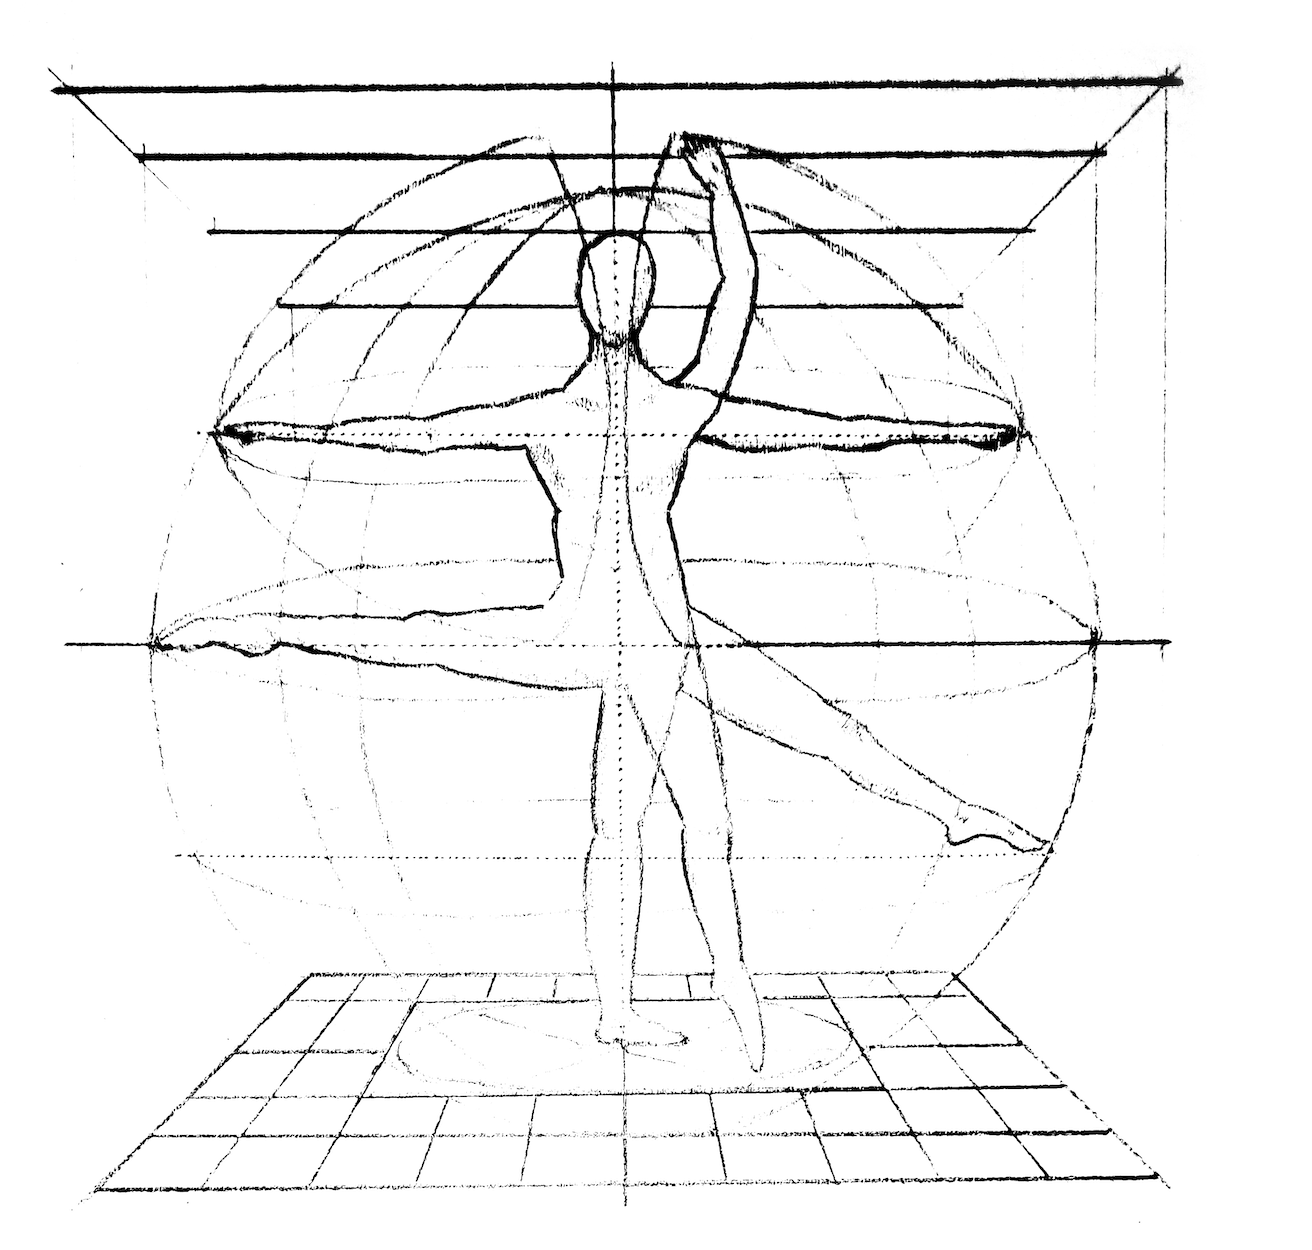
\includegraphics[height=2.5in]{images/#1/cover}}
        \end{center}\label{img:#1}
    \end{figure}
}

%%%%%%%%%%%%%%%%%%%%%%%%%%%%%%%%%%%%%%%%

\title{Crash Course Contact}
\date{\today}
\author{Christoph Pickl}

\usepackage{glossaries}

\makeglossaries

% USAGE: \gls{entryname}

\newglossaryentry{bigspace}{name=big space,description={A.k.a. ``big body''; A bit of a metaphysical word to reference the heightened awareness of all the people within a room. The emergent entity created by a group which comes together}}
\newglossaryentry{body-surfing}{name=body-surfing,description={One person rolling on the floor, and the other rolling over}}
\newglossaryentry{centergravity}{name=center of gravity,description={Literally the physical center of mass, somewhere in your lower belly area. Useful when trying to stay grounded and basing your partner during a lift to make yourself stable}}
\newglossaryentry{centerleviathan}{name=center of leviathan,description={An idea of becoming light, pulling from your sternum. Useful when being lifted in order to make yourself light}}
\newglossaryentry{goodgorilla}{name=good gorilla,description={Having a hollow back and the head above the ass as the base during a lift; part of our local jargon.}}
\newglossaryentry{guardianangel}{name=guardian angel,description={a third person for safety reasons to safeguard that there will be no injuries}}
\newglossaryentry{inertia}{name=inertia,description={the "lazyness" of an object, as defined by Newton's first law}}
\newglossaryentry{jam}{name=jam,description={a social event where usually a group of local people frequently come together to dance with or without (live) music}}
\newglossaryentry{kinesphere}{name=kinesphere,description={the personal space around us within reaching possibilities of our limbs without changing position}}
\newglossaryentry{kinesthesia}{name=kinesthesia,description={awareness of position and movement}}
\newglossaryentry{momentum}{name=momentum,description={when a physical object is moving with a certain speed}}
\newglossaryentry{negativespace}{name=negative space,description={the empty space which is not occupied by matter which can be "danced in", similar to \gls{kinesphere}}}
\newglossaryentry{over-dancer}{name=over-dancer,description={Synonym for ``flyer'' in other disciplines; the person who is being lifted by another person.}}
\newglossaryentry{proprioception}{name=proprioception,description={the ability to sense one's own body position}}
\newglossaryentry{roundrobin}{name=round-robin,description={a group practice, usually done during \gls{jam}s, some people dancing in the middle, others witnessing, and voluntarily changing roles}}
\newglossaryentry{skinesphere}{name=skinesphere,description={the space beneath the skin, as opposed to the kinesphere, refering to the inward focus involved in somatic preparations}}
\newglossaryentry{smalldance}{name=small dance,description={tiny, unconscious body reactions/movements to maintain balance/stand upright}}
\newglossaryentry{thebox}{name=the box,description={Basically the torso, the whole upper body and everything between shoulders and hips, with which most of the contact/sharing weight is engaged, excluding the limbs and head}}
\newglossaryentry{under-dancer}{name=under-dancer,description={Synonym for ``base'' in other disciplines; the person who is lifting another person.}}
\newglossaryentry{vector}{name=vector,description={a force with strength and direction, usually visualized as an arrow with a certain length}}


\begin{document}

\begin{titlepage}
\begin{center}
	
	\vspace*{\fill}
	
	\fontsize{22}{0}\selectfont
    {\sffamily CRASH COURSE CONTACT}
	\vskip 5mm
	%\rule{\textwidth}{0.4pt}
	\rule{84mm}{0.4pt}
	\vskip 1mm
	\fontsize{15}{22}\selectfont
	{\sffamily Small Steps into \\ the Wonderful World \\ of Contact Improvisation}
	
	\vskip 70mm
	
	\vspace*{\fill}

	\fontsize{9}{0}\selectfont
	{\sffamily 1st Edition - \today}
\end{center}
\end{titlepage}

\pagestyle{empty}
\tableofcontents
\clearpage
\ifodd\value{page}\else
  \thispagestyle{empty}
\fi

\pagestyle{fancy}

~

\vfill
\begin{center}
	\textit{Moving in unity.}\\
	\textit{In eternal spirals.}\\
	\textit{Guided by the moment.}
\end{center}
\vfill
\newpage
\chapter{About}\label{ch:about}

\chapterCoverImage{about}

So what is this book about, and where is its emphasis?
For whom is it written, and what is the person's background who has written it?
Finally, I also want to provide some general remarks as a form of a disclaimer before you continue reading.

\section{Book}\label{sec:book}

\begin{displayquote}
    ``\textit{Alles was gelernt werden kann, ist nicht wert gelehrt zu werden.}'' -- my older brother
\end{displayquote}

% History; intention, motivation
The following pages were initially written for the sole purpose of taking \textbf{personal notes} of my own experience, thoughts and insights.
After some time, it started to grow bigger and bigger, until it reached a level where it could also be of use to others.
Interesting also, that most of the questions being asked from beginners are the same, which means it is easily possible to satisfy that curiosity with a predefined set of answers.
Over many years, collecting from those sources, a structure would emerge, and that's how this book got its shape and (physical) manifestation.

% Emphasis; goal, USP
Looking at the other -few- books about Contact Improvisation (or short: CI) on the market, it seemed to me there was something missing for me.
A \textbf{structured approach} to the technicalities, the rules and principles explained in details, using less of the imaginary language but something an engineering mind can better relate to.
Furthermore, I had the need to make the \textbf{implicit norms and rules} in a delicate, social context such as created during a CI event, explicit.
This would allow people reading this book to safely navigate through the space without bumping and crossing on or the other boundary, without crash-landing, neither physically nor psychologically.

% Target group
Whether you consider yourself a \textbf{beginner or advanced} practitioner, I feel certain that you'll find something of value to you.
Being interested in getting more acquainted with the \textbf{theoretical background} -- next to your regular practice in the studio -- of this fine art is the only prerequisite.

\subsection{Disclaimer}\label{subsec:disclaimer}
%%%%%%%%%%%%%%%%%%%%%%%%%%%%%%%%%%%%%%%%%%%%%%%%%%%%%%%%%%%%%%%%%%%%%%%%%%%%%%%%%%%%%%%%%%%%%%%%%%%%%%%%%%%%%%%%%%%%%%%%

The book uses the \textbf{masculine version} when using examples for the sake of simplicity, in case both can be applied, and of course, always implying that the female version could have been equally used as well.

The book is \textbf{incomplete}, as any form of completeness can never be achieved anyway; we are not dealing with a hard science here.
I'd like to ask you to be gentle when you encounter an attempt of enumerating possibilities where you know that something is missing.
If you do so, please consider contacting me, contributing to this little project, and bringing it closer to completion and perfection, yet knowing we will never reach it, an asymptotic goal.

Whatever is written on the following pages does not claim to hold any absolute, objective truth.
Some parts are summaries of sources found along a path of exploration, whether they might be (direct or indirect) oral teachings, or written information found in books or on the internet.
Most of it is just a very \textbf{personal, subjective} collection of experiences, thoughts, associations, observations and opinions which were gathered along a single person's journey.
The content is, of course, also biased, although I made my best to free myself from my own limitations of reality-perception.
The content, thus, will sometimes be colored by my own personal background.
I shall be forgiven for my flawed, limited human nature.

\begin{displayquote}
    ``\textit{You are entitled to your opinion but you are not entitled to your own facts.}'' -- Daniel Patrick Moynihan
\end{displayquote}

It is said that there are no books existing written by a true master.
The reason being, that a master knows that it is impossible to capture the essence of a system in words, in a linear expression.
It happens sometimes, though, that students try to do that for the master, transcribing his teachings themselves.
I shall be forgiven for being such a student, desperate enough to achieve the unachievable in my own ignorance.

\section{Myself}\label{sec:myself}

To understand a system, we first need to understand its context and history.
If you want to understand psychoanalysis, for example, you first have to understand Sigmund Freud and the sociocultural environment he grew up in.
We are all just children of our time, and our views are shaped by it.
My own background will severely influence my approaches and values, ultimately also the content in this book.

\begin{displayquote}
    ``\textit{Good Kung-Fu looks bad, only bad Kung-Fu looks good.}'' -- my Aikido teacher
\end{displayquote}

My background is mainly rooted in the internal \textbf{martial arts} from Asia, and as such, my focus lies more on a practical approach (\textit{form follows function}).
For me, it is less about the aesthetics of movement, which might be more important for someone who is performing for others on stage, but more about the technical aspects.
``Right'' is what works in the most \textbf{pragmatic} way, meaning efficient in time and space, going into subjects like physics and biomechanics.
Whatever is within the principles of a system could also be considered is ``right'', relative to those principles, yet not necessarily ``better'' in every regard.

Besides those more physical aspects, the \textbf{psychological aspect} also has an important role to me.
The benefit for one's mental health, the ability to get to know oneself and others more deeply.
And, of course, a more philosophical/spiritual path which can also be walked with the help of this deep art.

As a body worker, I emphasize the importance of the non-verbal communication aspect which is happening while two people moving together.
The slowness, the gentleness in establishing a \textbf{deep connection} through listening, and the expressions of our personalities through this practice.

If you want to contact me, please feel free to do so by emailing me: \href{mailto:christoph@crashcoursecontact.org}{christoph@crashcoursecontact.org}

\section{Definition}\label{sec:definition}


CI is something that doesn't want to be defined, and thus confined, limited in what it can be.
It wants to stay open, to be able to be what the people need it to be.
It's by design something that you can't grasp properly, leaving you with the feeling you might have after watching a movie with an open ending.
It stays a mystery.
Yet we will try in this chapter to reveal the secret, take you backstage, and tell you the secret of the magician, how he's doing it.

\subsection{Essence}\label{sec:essence}
%%%%%%%%%%%%%%%%%%%%%%%%%%%%%%%%%%%%%%%%%%%%%%%%%%%%%%%%%%%%%%%%%%%%%%%%%%%%%%%%%%%%%%%%%%%%%%%%%%%%%%%%%%%%%%%%%%%%%%%%

Without a proper definition of what something is, without capturing its essence, it can't be properly talked about.
How does it relate and especially separate itself from other similar systems?
What are its \textbf{goals and principles}, so we can always check whether a specific method or direction is in alignment with these goals and principles.
Not necessarily that it would be wrong, but just to be aware when we step out of our system, and step into something (completely) different.
Communication is usually loaded with misunderstandings, and by having a \textbf{clear, mutual understanding} of what it is we are actually referring to, we can create more harmony in our interaction through clarity (of words).

So what is CI (sometimes also called \textit{contact} or \textit{contact dance} in the community) \textbf{compared} to other systems?
A dance, a sport, a (visceral) art-form or post-modern art-sport, partner acrobatics or martial arts?
Well, maybe all of it or none of it, or perhaps depending on how you approach it and what your background is and where you put the emphasis on.
Let's take a look at the different views on it, and by also looking at its history, it might get clearer what it is, or what it can be for you.

\subsection{By Comparison}\label{sec:by-comparison}
%%%%%%%%%%%%%%%%%%%%%%%%%%%%%%%%%%%%%%%%%%%%%%%%%%%%%%%%%%%%%%%%%%%%%%%%%%%%%%%%%%%%%%%%%%%%%%%%%%%%%%%%%%%%%%%%%%%%%%%%

Most of the emphasis is put on the following areas:

\begin{itemize*}
    \item [] \textbf{Experimental dance} -- practice-based research in dance labs
    \item [] \textbf{Theatrical form} -- improvised performances and lectures
    \item [] \textbf{Educational tool} -- training for dancers in improvisation
    \item [] \textbf{Awareness practice} -- listening skills for the subtleties in contact
    \item [] \textbf{Social dancing} -- at informal gatherings called ``jams''
\end{itemize*}

At its core, it involves \textbf{mindfulness}, sensing and collecting information which requires full presence and attention.
Thus, it could be considered a ``relational mindfulness practice in movement''.

\subsubsection{Dance}\label{subsec:dance}

It could be considered a form of improvised partner dancing, embedded in contemporary and (post-)modern dance.
Dance improvisation existed already before CI, but it didn't have the contact aspect as CI has, and especially not the ``\textit{shared point of contact}'' principle.
The development in dance history started with ballet, to modern (Martha Gram, John Cage, Cunningham), and then towards contemporary -- improvisation became not only a research tool, but a performance itself.
Those are mostly vertical, meaning standing, without any floor work involved; whereas in CI, we roll over each other on the floor, something which would be seen as rather unusual in other styles.
We use a \textbf{three-dimensional} spherical space, where every body-part can be a foot -- and be pushed against the ground.
We dance by ourselves, with a partner, or with multiple partners; we engage, re-engage, and dis-engage at our own will without clear structures.

% IMPROVISATION
CI is an \textbf{improvised} ``art-form'' (or ``art-sport''), thus without any predefined choreography.
Sometimes CI is used in choreographies, which is then called ``partnering''.
CI is an exploration, a way to try to ``break the system'' as it is improvised.
Nevertheless, CI is not something you would see in the professional dance world, a world where they are walking with very ``nice movements''.
The improvised nature of CI shifts the attention very much on listening and avoiding forcing a plan.
There is usually not enough time to follow along a plan, as the window closes very quickly again for a potential move to happen.
And yes, it is even related to other improvisation practices like improvisation acting: the ``Yes, and \ldots''-concept expressed just physically.

It is not so much that as a CI practitioner, you are serving the \textbf{audience} (in a performance), but rather that the audience is joining you.
It's about getting a visceral reaction from the audience of an improvisation art-form, that they want to join.
Ultimately, there is no difference between dancers and the audience, no hierarchy exists.

% MUSIC
The connection is also mostly with the partner, and less with the \textbf{music} being played.
Sometimes, and originally, there is even no music at all playing.
With regular partner dancing, both synchronize together via the help of music, having the focus on the music and musicality.
In CI we sync with each other through the connection we establish through deep listening, and the focus is on the moment, and the interaction.
If there are songs being played, they are usually more in the background, lacking vocals and a prominent drumset.
We let the people be the navigator and the driver, a free form expression without the restrictions, limitations or manipulations of the music's quality.

% GENDERS
It is distinct from other partner dance styles, as those are more focused on the social aspect, whereas CI comes from the art world.
Many other dance forms have also very strict \textbf{gender roles}, where usually the man would lead, and the woman would follow; exceptions exist, like, for example, Lindy Hop, a form of Swing, the mother of Rock'n'Roll.
In CI, everyone dances with everyone, without any clearly defined role, a totally egalitarian system.

% PHYSICAL
CI has a strong focus on the \textbf{physical} aspect: How to survive a high-impact volume, which leads to either a crash or a fall?
Lindy Hop has, for example, also some aspects of acrobatics, which Zouk also has a little bit.
Thinking about taking/lifting people on your body, on your core, your center.

% CONTACT
Next to the obvious improvised nature of CI, the contact quality plays the other important role.
Question being: Does contact always require constant, physical contact, as in touching?
In more old-school CI there was lots of play with impact, with distance and closeness.
Today, there is more the tendency to stay permanently in contact, and if distance happens, it would usually mean the end of the dance.
Sometimes you can question and challenge this attitude.
Keep dancing in the \gls{negativespace}; engaging, disengaging; maintaining a more mental connection with your partner in the distance.

% AESTHETICS
There is also a difference in styling, as many \textbf{aesthetically} pleasing dance styles would ``dress to impress''.
In CI, we would typically come wearing our pyjamas (pajamas), sloppy, cozy, comfy, pragmatic.
As we have no audience, there is no performance, thus there is no urge to perform.
We are who we are, whether it looks good or not is not of relevance.
Maybe even not whether it has ``internal aesthetics'', whether it feels good, but just to feel itself with a non-judgmental mindset, welcoming what is, and experience some sort of satisfaction instead in this depth.

\subsubsection{Martial Art}\label{subsec:martial-art}

It is also combined with some minor aspects of eastern philosophy and a few things from the 1960s hippie culture.
The reason is that some founders of CI had their background in the Japanese martial art of \textbf{Aikido}, which is similar to Brazilian Ju-Jitsu.
Gently receiving incoming force and deflect it in circular movements, not resisting but rather listen, perceive, interpret and work with what's there at the moment.
Connecting with one's weight, one's center (''\textit{hara}`` in Japanese) and acting from that place.
By listening and using ``what is'', we can move with less effort.
Acting below the level of voluntary muscular contraction, a preliminary state, being prepared.
The joints and the whole state of being stimulated, readied for action.

Yet of course, CI totally lacks the intention of it being even remotely applied in a contest or let alone in a street fight.
There is no emphasis put on practicality during a physical conflict, still having skills in, for example, rolling (Judo) can be extremely useful.

We could also use the metaphysical, philosophical concept of Ki (or ``Qi'' in Chinese), which expresses itself in the quality and potential of connections.
It's active in an ideokinetic way, as an image-effect, which influences the course in which events might develop.
It is the potential of the extension-principle, a source, or better ``a radiation'' of energy within the body.

\subsubsection{Sports}\label{subsec:sports}

If we define sports of any form of physical activity, then CI (as like any other dance form), is for sure a sport.
Yet, sports usually has an ego-benefitting aspect by being able to measure performance and even having competitions where people/teams compete against each other -something totally missing in CI, yet not in most dance forms.
Sports also usually lacks the depth, the possibilty for ``soul exploration'' and spiritual growth which also has often an emphasis in CI.

\subsubsection{Acrobatics}\label{subsec:acrobatics}

The main founder, Steve Paxton himself, was a \textbf{gymnast}, and that might be the reason why still some of CI resembles more \textbf{partner acrobatics} than dancing.
The many (demanding) lifts, and the high velocity and high-impact movements can require a high level of fitness of the practitioners, just like acrobats do.
Whereas proper partner acrobatics goes way beyond what CI is doing, in terms of physical demands and risky techniques.

Acrobatics is Greek (\textit{akrobatéō}) and means to ``walk on tiptoe'', to strut.
The geometry of aerobatics is a combination of aeroplane and acrobatics, to fly and to tiptoe.
We use bodies, instead of airplanes, thus it would be more correct to call it ``bodatics'' or ``somatics'' maybe?

\subsubsection{Applied Physics}\label{subsec:applied-physics}

CI is an exploration / research practice of the \textbf{physical forces} of one's body in relationship to others by using the principle of sharing weight, touch, and movement awareness, while moving in contact and on the ground.
To play with the artistry of falling unbalanced and counterbalance, with gravity and physics.
To learn the mechanics of the body to handle someone's weight or to be lifted, along with breathing techniques.
Alternatively, it can be stated:

\begin{center}
    ``\textit{CI is a three-body-problem with two dancers, being shaped and moved by momentum, gravity, and force, dealing with the third body, the ground.}''
\end{center}

\subsection{Historically}\label{sec:historically}
%%%%%%%%%%%%%%%%%%%%%%%%%%%%%%%%%%%%%%%%%%%%%%%%%%%%%%%%%%%%%%%%%%%%%%%%%%%%%%%%%%%%%%%%%%%%%%%%%%%%%%%%%%%%%%%%%%%%%%%%

In the early beginnings, in the 1970s, every time the founding members practiced CI, they would redefine it, asking the very same question over and over again: ``What is CI \textit{now}?'' An early definition by \textbf{Steve Paxton} and others was (source: CQ Vol. 5:1, Fall 1979):

\begin{displayquote}
    ``A continuously evolving system of improvised movement.
    Two bodies, communicating with each other in physical contact, creating a relationship with the physical laws (motion, gravity, momentum, inertia).
    Sensitive, thus relaxed of unnecessary muscular tension, and willing to experience a natural flow.
    Techniques may include: Rolling, falling, being upside-down, following, supporting and giving weight.

    A physical dialogue ranging from stillness to highly energetic exchange.
    Alert enough to stay in an energetic state of physical disorientation, trusting your survival instincts.
    A free play seeking for balanced movements, leading to a physical and emotional truth, shared currently, leaving you informed, centered, and enlivened.''
\end{displayquote}

\subsection{Possible Definitions}\label{sec:possible-definitions}
%%%%%%%%%%%%%%%%%%%%%%%%%%%%%%%%%%%%%%%%%%%%%%%%%%%%%%%%%%%%%%%%%%%%%%%%%%%%%%%%%%%%%%%%%%%%%%%%%%%%%%%%%%%%%%%%%%%%%%%%

Definitions, and the same with any terminology, are time-, space- and person-dependent.
Just as with the improvised nature of CI, it is a constantly moving target.
By asking the same question a week later, the answer you receive will already be different.
And as such, the answer you will give to yourself, what CI is for you, will and most likely also should change, as you yourself are in constant change.

There is still a rough \textbf{body of agreement} -- a congruent understanding -- of what it is, and what it is not, leading to a definition stable across time, space, and practitioner.
It's like a tree: The trunk which are the agreed principles, and it's branches and leaves (the styles/adaptations) representing the edges where you can play freely.

\textbf{Steve Paxton} himself stated in 1979:
\begin{displayquote}
    ``The exigencies\footnote{exigency = a pressing or urgent situation, requirement, or need} of the form dictate a mode of movement which is relaxed, constantly aware and prepared, and on flowing.
    As a basic focus, the dancers remain in physical touch, mutually supportive and innovative, meditating upon the physical laws relating to their masses: gravity, momentum, inertia, and friction.
    They do not strive to achieve results, but rather, to meet the constantly changing physical reality with appropriate placement and energy.''
\end{displayquote}

\textbf{Nancy Stark Smith} once mentioned:
\begin{displayquote}
    ``It resembles other familiar duet forms, such as the embrace, wrestling, surfing, martial arts, and the Jitterbug (Lindy Hop and swing dances), encompassing a wide range of movement from stillness to highly athletic.''
\end{displayquote}

\textbf{Daniel Lepkoff} states about the core of CI:
\begin{displayquote}
    ``To put focus on bodily awareness and physical reflexes, rather than consciously controlled movements.
    Precedence of body experience first, and mindful cognition second, is an essential distinction between CI and other approaches to dance.''
\end{displayquote}

\textbf{Ray Chung} once announced in a workshop 2009 that:
\begin{displayquote}
    ``CI is an open-ended exploration of the kinesthetic possibilities of bodies moving through contact.
    Sometimes wild and athletic, sometimes quiet and meditative, it is a form open to all bodies and inquiring minds.''
\end{displayquote}

\subsection{Beyond CI}\label{sec:beyond-ci}
%%%%%%%%%%%%%%%%%%%%%%%%%%%%%%%%%%%%%%%%%%%%%%%%%%%%%%%%%%%%%%%%%%%%%%%%%%%%%%%%%%%%%%%%%%%%%%%%%%%%%%%%%%%%%%%%%%%%%%%%

CI is for sure not a pure \textbf{martial art}, as it has no claim to have any practical fighting application.
Nor is it a competitive \textbf{sport} in any way, as there are no competitions and due to its artistic nature it would be difficult, or at least without much meaning, to judge one as being better than the other.
It has many aspects of partner \textbf{acrobatics}, but lacks many technical possibilities due to the nature of its principles.

It is also not really your regular \textbf{dance} form like Salsa or Tango, due to several reasons: We don't dress (nor dance) to impress but rather show up with our authentic selves; we don't move to only look good or aesthetically (to others); we focus more on the internal and interpersonal aspects than the external ones; we often dance without music; there are no real techniques which can be learned but only guiding principles from which some specific movements can emerge.

As it is the case with so many (or maybe even all?) disciplines: Once the rule has been understood, and you know what you are doing, it can be broken by the student, thus \textbf{becoming a master} of it.
Finally, it has to be mentioned that a system\footnote{In this case we talk about CI as a system, but the forementioned wisdome can be applied to our world's system, politically or economically, to technology, to our endless todo lists \ldots} is supposed to be of service to the user (not the other way round), and its boundaries and dogma should not limit but enrich the applicant.
Whenever the purpose is hindered by the system, the system shall be left behind, and we should remember the original goal which was there in the first place, and not to serve the gods we created.

\section{Community}\label{sec:community}

The term ``community'' is in some areas used for people living in the same place, something hippies would do who strive for a more ``natural'' approach to life, people who drop out the system, sharing knowledge about each other, rather than about a specific \textbf{practice}, and helping each other in times of need.
And there is even a current trend in our society that companies are using phrases like ``Come, join the family!'' which even deludes the word family very much.

We use the term ``community'' here for a group of people \textbf{sharing} the same passion for this practice, and getting curious about the other person, from a very basic physical connection.
Sometimes this curiosity goes to their life, experiences, and ideas, which sometimes can lead to afterward also sharing food; from there, friendship can happen.
Sometimes it is also just a great dance partner, but personally, we might have nothing in common, and we also do not want to become friends.
We see each other as ``only dance partners'', and the depth of care we feel is a bit less than, for example, for our beloved neighbor.

In the CI ``community'' this is a bit off though (compared to regular dance scenes), as when someone discontinues to come to classes or jams after a while, we might not be real friends, yet we would still reach out for each other, asking where he is, \textbf{helping} each other out (with health issues, financially) and support if needed.
This happens especially in smaller classes, where there is more of a sense of community.
These silos also happen according to the attitude of the teacher or the jam, where people will converge into specific places; norms will differ based on that.

People who practice or teach CI believe in what they do, in the goodness that it gives the world.
They want to expand the pool to reach more people, and that's why you will see little competition and more \textbf{collaboration} in the scene.
Maybe there will be a bit more competition if it's one's only source of income, a scarce modality; instead of CI being a livelihood, a hobby, a passion.
Some teachers will invite guest teachers, or send their students to another teacher, to a different city, or a teacher who is more technical or in some other way different.
There is not much ``fighting'' among CI practitioners happening, but also collaboration are not so often happening, as it is a very \textbf{individual practice}.
There are festivals, where (abroad) teachers are being invited, but usually when invited, then not by other teachers but by schools, institutions, or organizers.
The norm is nevertheless a ``city-based'' teacher who offers 2--3 classes a week, and sometimes there are ``travelling teachers''.
And there is also a win-win-win in having different student-teacher relationships in one's own workshop.

\subsection{Jams}\label{sec:jams}
%%%%%%%%%%%%%%%%%%%%%%%%%%%%%%%%%%%%%%%%%%%%%%%%%%%%%%%%%%%%%%%%%%%%%%%%%%%%%%%%%%%%%%%%%%%%%%%%%%%%%%%%%%%%%%%%%%%%%%%%

There is a broad, global community that regularly organizes social dances, so-called ``\gls{jam}s''.
You will see that many of those people also often overlap with the Ecstatic Dance communities\footnote{Many people from Ecstatic Dance say that they have done ``contact'' but what they are doing and their idea has little to nothing to do with CI. This confusion is about ``touch-based partner dance'' versus the art-form of CI (sharing weight, etc.). Those people might also bring in a slightly different (sensual-sexual, maybe even Tantric) attitude which is not welcome in CI.}.
Jams are \textbf{social gatherings} without a leader, yet sometimes with someone who facilitates it; similar to jazz jam sessions or Milongas in Tango.
It's an opportunity to practice \textbf{freely}, where people can meet and negotiate together their dance, or observe the practice of their partners.
It's an occasion to meet other fellow practitioners, friends or strangers, old, young, experienced, and novice, and has a bit of a taste of being a hybrid between bodily meditation, psycho-kinesthetic therapy, sports training and a dance improvised session.
They can be regularly in a studio for a few hours, or longer retreat jams for several days in spring resorts where it can be practiced at any hour of the day.

Sometimes you will encounter that the \textbf{facilitator} takes a bit more the lead, by hosting sharing circles at the beginning and/or at the end, and by providing some warm-up exercises.
Sometimes you will have a playlist providing musical background throughout, sometimes you might even encounter a live musician.
Yet, traditionally jams are being kept \textbf{silent}; to let fully unfold of what is alive presently between the dancing partners; to not let the music dictate externally but allow for full expression of what's present, as one of my dance teachers once said:

\begin{displayquote}
    ``\textit{Music makes a dancer stupid.}'' -- my dance teacher's teacher
\end{displayquote}

At the end (also sometimes in classes/workshops), you will sometimes participate in an exercise called ``\textbf{\gls{roundrobin}}''.
Usually two, three or four couples (or sometimes half of the people) are constantly in the center of the room, dancing.
The rest of the people are sitting on the edge, holding space, being present, giving in their energy.
As an active witness, you might learn something, or at least get inspired by simply observing.
When you enter and join a couple, another person is leaving, so the number of people stays constant throughout.

\subsection{Stereotype}\label{sec:stereotype}
%%%%%%%%%%%%%%%%%%%%%%%%%%%%%%%%%%%%%%%%%%%%%%%%%%%%%%%%%%%%%%%%%%%%%%%%%%%%%%%%%%%%%%%%%%%%%%%%%%%%%%%%%%%%%%%%%%%%%%%%

There is no clear stereotypical, \textbf{physical appearance} for so-called ``CI people'', as we might have when thinking of people who do Yoga, Hip Hop, or Tantra.
CI practitioners are nevertheless quickly spotted on the dance floor, not so much based on their looks but how they move, how they engage, their behavior with weight.
There appears to be a mutual, unconscious ability to spot each other on the dance floor, which makes them find each other rather quickly -like magic.

A stereotypical CI practitioner is often wearing common \textbf{dance clothes}, nothing too casual or street clothes, but also nothing too fancy.
The age range is rather big, yet for the technical part it's usually around 25--45.
Socioeconomically, it's a little bit on the higher end, meaning people who are \textbf{financially} a bit better off.
Teachers might be willing to give a discount to people who can't easily afford to pay for the classes/workshops, so in case needed, feel free to go ahead and ask, as the worst thing you could get is a ``no'' and in the best case you can afford to go for your dream.
Also, strictly \textbf{religious} people seem not to be attracted by it, most likely because of the touch and the physical proximity.

CI people have no need to attach themselves to a \textbf{subculture} and shape their personality around it; there is no need for ``another stamp'' as is seen so often in other practices.
CI is about the \textbf{physicality}, and less a ``spiritual practice for personal growth'', or a community, as stated above.
Still, the way we move might influence our personality; similar to the increased sensuality when moving Tango, but that's not a big thing in CI\@.
It's very \textbf{egalitarian}, meaning no roles, and a plain physical form.
It's more \textbf{technical}, more raw, and no (moral) values are being conveyed -whereas the egalitarian approach might be a value in itself.
Not only that, but it is \textbf{independent} of sex, gender, age, and body; there is no leading nor following based on sex or gender -just play.
Furthermore, it doesn't convince others of the greatness of CI, although everyone is invited and welcome to join -it's fun.

\section{History}\label{sec:history}

As a theoretical book about a practiced system, we will cover how it all started and the people involved.
A bit of a ``who is who'' and how it is set up in terms of institutions and organizations.
By knowing its origin, and how the way CI is done currently, it will allow you to understand the differences.
We will finish up with a bit of an outlook and wishes for the future of it.

``\textit{To know who you are today, I need to know your past, and maybe even can predict something about your future.}''
This applies not only to individuals, but as well to humanity as a whole and localized phenomena like the art of CI itself.
By knowing its origins, we can prevent from diverting too far from it, and reach a more profound understanding of why things are the way they are.
And also, of course, to nourish an attitude of honor, paying our respect to the founding fathers—and mothers.
To create some tradition, something our society these days so much lacks and yet is so much in need of -- even though it might not be aware of it.

\subsection{Founding Parents}\label{subsec:founding-parents}
%%%%%%%%%%%%%%%%%%%%%%%%%%%%%%%%%%%%%%%%%%%%%%%%%%%%%%%%%%%%%%%%%%%%%%%%%%%%%%%%%%%%%%%%%%%%%%%%%%%%%%%%%%%%%%%%%%%%%%%%

% TODO drawing of paxton&stark

CI was developed in June \textbf{1972} in the US by mainly a man called \textbf{Steve Paxton}, ``the father of CI'' -- see his picture on the right --, who was an American dancer, gymnastics and choreographer and former Aikidoka (someone who practices the Japanese martial art Aikido) who lived in New York City (by that time mainly performing in the Judson Dance Theater).
He was keen to explore and push the boundaries to develop this new practice, some sort of ``art-sport''.

Next to him, it is worth mentioning \textbf{Nancy Stark Smith} -- ``the mother of CI'' --, who is the one still holding CI, as Steve stopped doing CI about 7 years after its invention, intending to give it to the people.
She continued with another partner and started the Contact Quarterly magazine, a vehicle to share ideas, to hold the theme and practice of CI\@.

\subsection{Creation}\label{subsec:creation}
%%%%%%%%%%%%%%%%%%%%%%%%%%%%%%%%%%%%%%%%%%%%%%%%%%%%%%%%%%%%%%%%%%%%%%%%%%%%%%%%%%%%%%%%%%%%%%%%%%%%%%%%%%%%%%%%%%%%%%%%

In spring 1972, Steve Paxton invited a group of 17 students and colleagues, dancers, martial artists, acrobats, gymnasts and athletes, to explore and research the \textbf{extremes of movement and disorientation} -- from standing still to falling, rolling, colliding and jumping in the air -- in a two-week workshop.
While moving with high velocity, running into each other, bumping, trying to survive, and see what the result will be.\footnote{A little bit like what they do at the Large Hadron Collider at CERN: Smashing some particles at each other and be excited about what would happen.}

He wanted the dancers to work with him on the form he was evolving, and at the end of this week of residency, the group presented a performance named ``Contact Improvisation''.
To see for yourself how those first steps looked like, watch this old black-white recording from 1972: \url{https://www.youtube.com/watch?v=9FeSDsmIeHA}

Out of that exploration, a 20-minutes performance piece called ``\textit{Magnesium}'' arose, whereas the first quarter-hour was about jumping and bumping, manipulation and clinging.
Only the last 5 minutes, the so-called ``\gls{smalldance}'' was performed: A form of meditation that is practiced standing, where attention is paid to postural adjustments and micro-weight transfers.
Videos narrated by Steve about that are available, which are very much encouraged to watch, to also see the progression from those impactful years of '72, '75 and '87.

\subsection{Institutionalization}\label{subsec:institutionalization}
%%%%%%%%%%%%%%%%%%%%%%%%%%%%%%%%%%%%%%%%%%%%%%%%%%%%%%%%%%%%%%%%%%%%%%%%%%%%%%%%%%%%%%%%%%%%%%%%%%%%%%%%%%%%%%%%%%%%%%%%

At first, around 1975, it was considered to \textbf{trademark} the term Contact Improvisation, but this idea was rejected in favor of establishing a forum for communication, which nowadays is the website of \href{https://contactquarterly.com}{Contact Quarterly} and is still co-edited by Nancy Stark Smith herself.
So it was never \textbf{institutionalized}, nor was the name \textbf{copyright} protected.
Together with \href{http://www.ecite.org}{ECITE} (the European Contact Improvisation Teachers Exchange), those two can be considered the main international forums ensuring the quality and continuation of CI\@.

The decision was very deliberate to not have any form of legal institute or \textbf{certifications}, free of any hierarchy.
Remember that a certificate usually doesn't mean that that person is good, but just that the certification was passed.

The downside of not having an authority verifying the competence of the teachers is, of course, that when the word was spreading, more and more \textbf{injuries} started to happen; that's why: ``\textit{One should never teach what one doesn't know properly}''.

\subsection{Further Spreading}\label{subsec:further-spreading}
%%%%%%%%%%%%%%%%%%%%%%%%%%%%%%%%%%%%%%%%%%%%%%%%%%%%%%%%%%%%%%%%%%%%%%%%%%%%%%%%%%%%%%%%%%%%%%%%%%%%%%%%%%%%%%%%%%%%%%%%

A few years after the founding event, the very first ``Country Jam'' was organized in 1979, where about 50 people came together to freely exchange and dance, without any structure.
Neither a workshop, conference nor a seminar.
Just co-created being, dancing and living in flux.
Later on, it was introduced in new avant-garde (experimental artists) dance schools in the US\@.

The members of the founding group scattered across the US and started to teach the practice.
It became smoother, continuous and \textbf{controlled}, yet still avoiding eye and direct hand contact.
Much emphasize was put on the experience of flow, which is more of an aesthetic choice (Nancy Stark Smith), yet the central characteristics preserved.

\textbf{Europe} was presented with CI first 1873 in Italy, and later Steve Paxton and Lisa Nelson regularly went to the UK and Amsterdam (School for New Dance Development) as the transmission belts for CI in the whole of Europe.
Belgium was visited by Paxton since the 1980s, but apart to certain outbreaks of fever in successful jams, it didn't leave any lasting traces among dancers.

As founding people could be considered (next to Steve Paxton): Nancy Stark Smith, Danny Lepkoff, Lisa Nelson, Karen Nelson, Nita Little, Andrew Harwood, and Ray Chung.

For more detailed information, read books like \textit{Sharing the Dance} and others which you can find in the complementary online part of this book.

\subsection{Then and Now}\label{subsec:then-and-now}
%%%%%%%%%%%%%%%%%%%%%%%%%%%%%%%%%%%%%%%%%%%%%%%%%%%%%%%%%%%%%%%%%%%%%%%%%%%%%%%%%%%%%%%%%%%%%%%%%%%%%%%%%%%%%%%%%%%%%%%%

It was, for sure, very different back then, and that's why sometimes people would also refer to it as ``\textit{Old School Contact}''.
There was a \textbf{high risk} with very high velocity, and it, for sure, looked very amazing -and very scary too.
Good to know, though is, that they trained on \textbf{mats}, especially at the very beginning (see the videos), which would make the impact of falling much less.
After they started to do the same without mats, though, they got -- quite a lot of -- injuries.

In the last few decades, much more emphasis was put on \textbf{flow}, instead on ``explosion'', and also on figuring out the \textbf{least resistant} pathway.
Some people claim that CI lost quite a lot of its characteristics along the way, yet it could be said that it's nice to have both, to be able to choose what you want.
Being able to survive the explosion, and play comfortably in the flow.

Today there are many different \textbf{styles}: more flow, more impactful, acrobatics, dance, acting, \ldots
The differences are mostly based on the uniqueness of the teachers, along with their lineages; but also due to culturally specifics.
Some countries may have simply other ``body orientations'', resulting in a different CI style.

\subsection{Future}\label{subsec:future}
%%%%%%%%%%%%%%%%%%%%%%%%%%%%%%%%%%%%%%%%%%%%%%%%%%%%%%%%%%%%%%%%%%%%%%%%%%%%%%%%%%%%%%%%%%%%%%%%%%%%%%%%%%%%%%%%%%%%%%%%

Hopefully, it will keep a \textbf{strong trunk}, meaning: People keep on researching the practice, while still knowing where it comes from, knowing its roots.
We are all welcoming the \textbf{branches}, e.g.\ CI combined with other practices like ``Contact Tango'', ``Contact Beyond Contact'', and so forth, or CI with using substances for \textit{other states of awareness}.
Hoping for -- as the tree is branching -- that the main trunk will stay the main trunk so that there is no need for the distinction between ``I am a CI \textit{purist}'' but that it's possible to simply say: ``I'm doing CI''.
The trunk has been \textbf{stable} for the last 50 years, yet plenty of new branches appeared in the last 20 years; branches which merge different forms together.
It is important that people be aware that those branches and merges are not CI the way it is actually practiced.
And lastly, what's needed are good teachers, jams, and spaces where the ideas and principles are held from CI: Knowing the physical aspect but also keeping the history.


\chapter{Definition}\label{ch:definition}

\chapterCoverImage{definition}

CI is something that doesn't want to be defined, and thus confined, limited in what it can be.
It wants to stay open, to be able to be what the people need it to be.
It's by design something that you can't grasp properly, leaving you with the feeling you might have after watching a movie with an open ending.
It stays a mystery.
Yet we will try in this chapter to reveal the secret, take you backstage, and tell you the secret of the magician, how he's doing it.

\section{Essence}\label{sec:essence}

Without a proper definition of what something is, without capturing its essence, it can't be properly talked about.
How does it relate and especially separate itself from other similar systems?
What are its \textbf{goals and principles}, so we can always check whether a specific method or direction is in alignment with these goals and principles.
Not necessarily that it would be wrong, but just to be aware when we step out of our system, and step into something (completely) different.
Communication is usually loaded with misunderstandings, and by having a \textbf{clear, mutual understanding} of what it is we are actually referring to, we can create more harmony in our interaction through clarity (of words).

So what is CI (sometimes also called \textit{contact} or \textit{contact dance} in the community) \textbf{compared} to other systems?
A dance, a sport, a (visceral) art-form or post-modern art-sport, partner acrobatics or martial arts?
Well, maybe all of it or none of it, or perhaps depending on how you approach it and what your background is and where you put the emphasis on.
Let's take a look at the different views on it, and by also looking at its history, it might get clearer what it is, or what it can be for you.

\section{By Comparison}\label{sec:by-comparison}
%%%%%%%%%%%%%%%%%%%%%%%%%%%%%%%%%%%%%%%%%%%%%%%%%%%%%%%%%%%%%%%%%%%%%%%%%%%%%%%%%%%%%%%%%%%%%%%%%%%%%%%%%%%%%%%%%%%%%%%%

Most of the emphasis is put on the following areas:

\begin{itemize*}
	\item [] \textbf{Experimental dance} -- practice-based research in dance labs
	\item [] \textbf{Theatrical form} -- improvised performances and lectures
	\item [] \textbf{Educational tool} -- training for dancers in improvisation
	\item [] \textbf{Awareness practice} -- listening skills for the subtleties in contact
	\item [] \textbf{Social dancing} -- at informal gatherings called ``jams''
\end{itemize*}

At its core, it involves \textbf{mindfulness}, sensing and collecting information which requires full presence and attention.
Thus, it could be considered a ``relational mindfulness practice in movement''.

\subsection{Dance}\label{subsec:dance}

It could be considered a form of improvised partner dancing, embedded in contemporary and (post-)modern dance.
Dance improvisation existed already before CI, but it didn't have the contact aspect as CI has, and especially not the ``\textit{shared point of contact}'' principle.
The development in dance history started with ballet, to modern (Martha Gram, John Cage, Cunningham), and then towards contemporary -- improvisation became not only a research tool, but a performance itself.
Those are mostly vertical, meaning standing, without any floor work involved; whereas in CI, we roll over each other on the floor, something which would be seen as rather unusual in other styles.
We use a \textbf{three-dimensional} spherical space, where every body-part can be a foot -- and be pushed against the ground.
We dance by ourselves, with a partner, or with multiple partners; we engage, re-engage, and dis-engage at our own will without clear structures.

% IMPROVISATION
CI is an \textbf{improvised} ``art-form'' (or ``art-sport''), thus without any predefined choreography.
Sometimes CI is used in choreographies, which is then called ``partnering''.
CI is an exploration, a way to try to ``break the system'' as it is improvised.
Nevertheless, CI is not something you would see in the professional dance world, a world where they are walking with very ``nice movements''.
The improvised nature of CI shifts the attention very much on listening and avoiding forcing a plan.
There is usually not enough time to follow along a plan, as the window closes very quickly again for a potential move to happen.
And yes, it is even related to other improvisation practices like improvisation acting: the ``Yes, and \ldots''-concept expressed just physically.

It is not so much that as a CI practitioner, you are serving the \textbf{audience} (in a performance), but rather that the audience is joining you.
It's about getting a visceral reaction from the audience of an improvisation art-form, that they want to join.
Ultimately, there is no difference between dancers and the audience, no hierarchy exists.

% MUSIC
The connection is also mostly with the partner, and less with the \textbf{music} being played.
Sometimes, and originally, there is even no music at all playing.
With regular partner dancing, both synchronize together via the help of music, having the focus on the music and musicality.
In CI we sync with each other through the connection we establish through deep listening, and the focus is on the moment, and the interaction.
If there are songs being played, they are usually more in the background, lacking vocals and a prominent drumset.
We let the people be the navigator and the driver, a free form expression without the restrictions, limitations or manipulations of the music's quality.

% GENDERS
It is distinct from other partner dance styles, as those are more focused on the social aspect, whereas CI comes from the art world.
Many other dance forms have also very strict \textbf{gender roles}, where usually the man would lead, and the woman would follow; exceptions exist, like, for example, Lindy Hop, a form of Swing, the mother of Rock'n'Roll.
In CI, everyone dances with everyone, without any clearly defined role, a totally egalitarian system.

% PHYSICAL
CI has a strong focus on the \textbf{physical} aspect: How to survive a high-impact volume, which leads to either a crash or a fall?
Lindy Hop has, for example, also some aspects of acrobatics, which Zouk also has a little bit.
Thinking about taking/lifting people on your body, on your core, your center.

% CONTACT
Next to the obvious improvised nature of CI, the contact quality plays the other important role.
Question being: Does contact always require constant, physical contact, as in touching?
In more old-school CI there was lots of play with impact, with distance and closeness.
Today, there is more the tendency to stay permanently in contact, and if distance happens, it would usually mean the end of the dance.
Sometimes you can question and challenge this attitude.
Keep dancing in the \gls{negativespace}; engaging, disengaging; maintaining a more mental connection with your partner in the distance.

% AESTHETICS
There is also a difference in styling, as many \textbf{aesthetically} pleasing dance styles would ``dress to impress''.
In CI, we would typically come wearing our pyjamas (pajamas), sloppy, cozy, comfy, pragmatic.
As we have no audience, there is no performance, thus there is no urge to perform.
We are who we are, whether it looks good or not is not of relevance.
Maybe even not whether it has ``internal aesthetics'', whether it feels good, but just to feel itself with a non-judgmental mindset, welcoming what is, and experience some sort of satisfaction instead in this depth.

\subsection{Martial Art}\label{subsec:martial-art}

It is also combined with some minor aspects of eastern philosophy and a few things from the 1960s hippie culture.
The reason is that some founders of CI had their background in the Japanese martial art of \textbf{Aikido}, which is similar to Brazilian Ju-Jitsu.
Gently receiving incoming force and deflect it in circular movements, not resisting but rather listen, perceive, interpret and work with what's there at the moment.
Connecting with one's weight, one's center (''\textit{hara}`` in Japanese) and acting from that place.
By listening and using ``what is'', we can move with less effort.
Acting below the level of voluntary muscular contraction, a preliminary state, being prepared.
The joints and the whole state of being stimulated, readied for action.

Yet of course, CI totally lacks the intention of it being even remotely applied in a contest or let alone in a street fight.
There is no emphasis put on practicality during a physical conflict, still having skills in, for example, rolling (Judo) can be extremely useful.

We could also use the metaphysical, philosophical concept of Ki (or ``Qi'' in Chinese), which expresses itself in the quality and potential of connections.
It's active in an ideokinetic way, as an image-effect, which influences the course in which events might develop.
It is the potential of the extension-principle, a source, or better ``a radiation'' of energy within the body.

\subsection{Sports}\label{subsec:sports}

If we define sports of any form of physical activity, then CI (as like any other dance form), is for sure a sport.
Yet, sports usually has an ego-benefitting aspect by being able to measure performance and even having competitions where people/teams compete against each other -something totally missing in CI, yet not in most dance forms.
Sports also usually lacks the depth, the possibilty for ``soul exploration'' and spiritual growth which also has often an emphasis in CI.

\subsection{Acrobatics}\label{subsec:acrobatics}

The main founder, Steve Paxton himself, was a \textbf{gymnast}, and that might be the reason why still some of CI resembles more \textbf{partner acrobatics} than dancing.
The many (demanding) lifts, and the high velocity and high-impact movements can require a high level of fitness of the practitioners, just like acrobats do.
Whereas proper partner acrobatics goes way beyond what CI is doing, in terms of physical demands and risky techniques.

Acrobatics is Greek (\textit{akrobatéō}) and means to ``walk on tiptoe'', to strut.
The geometry of aerobatics is a combination of aeroplane and acrobatics, to fly and to tiptoe.
We use bodies, instead of airplanes, thus it would be more correct to call it ``bodatics'' or ``somatics'' maybe?

\subsection{Applied Physics}\label{subsec:applied-physics}

CI is an exploration / research practice of the \textbf{physical forces} of one's body in relationship to others by using the principle of sharing weight, touch, and movement awareness, while moving in contact and on the ground.
To play with the artistry of falling unbalanced and counterbalance, with gravity and physics.
To learn the mechanics of the body to handle someone's weight or to be lifted, along with breathing techniques.
Alternatively, it can be stated:

\begin{center}
	``\textit{CI is a three-body-problem with two dancers, being shaped and moved by momentum, gravity, and force, dealing with the third body, the ground.}''
\end{center}

\section{Historically}\label{sec:historically}
%%%%%%%%%%%%%%%%%%%%%%%%%%%%%%%%%%%%%%%%%%%%%%%%%%%%%%%%%%%%%%%%%%%%%%%%%%%%%%%%%%%%%%%%%%%%%%%%%%%%%%%%%%%%%%%%%%%%%%%%

In the early beginnings, in the 1970s, every time the founding members practiced CI, they would redefine it, asking the very same question over and over again: ``What is CI \textit{now}?'' An early definition by \textbf{Steve Paxton} and others was (source: CQ Vol. 5:1, Fall 1979):

\begin{displayquote}
	``A continuously evolving system of improvised movement.
	Two bodies, communicating with each other in physical contact, creating a relationship with the physical laws (motion, gravity, momentum, inertia).
	Sensitive, thus relaxed of unnecessary muscular tension, and willing to experience a natural flow.
	Techniques may include: Rolling, falling, being upside-down, following, supporting and giving weight.

	A physical dialogue ranging from stillness to highly energetic exchange.
	Alert enough to stay in an energetic state of physical disorientation, trusting your survival instincts.
	A free play seeking for balanced movements, leading to a physical and emotional truth, shared currently, leaving you informed, centered, and enlivened.''
\end{displayquote}

\section{Possible Definitions}\label{sec:possible-definitions}
%%%%%%%%%%%%%%%%%%%%%%%%%%%%%%%%%%%%%%%%%%%%%%%%%%%%%%%%%%%%%%%%%%%%%%%%%%%%%%%%%%%%%%%%%%%%%%%%%%%%%%%%%%%%%%%%%%%%%%%%

Definitions, and the same with any terminology, are time-, space- and person-dependent.
Just as with the improvised nature of CI, it is a constantly moving target.
By asking the same question a week later, the answer you receive will already be different.
And as such, the answer you will give to yourself, what CI is for you, will and most likely also should change, as you yourself are in constant change.

There is still a rough \textbf{body of agreement} -- a congruent understanding -- of what it is, and what it is not, leading to a definition stable across time, space, and practitioner.
It's like a tree: The trunk which are the agreed principles, and it's branches and leaves (the styles/adaptations) representing the edges where you can play freely.

\textbf{Steve Paxton} himself stated in 1979:
\begin{displayquote}
	``The exigencies\footnote{exigency = a pressing or urgent situation, requirement, or need} of the form dictate a mode of movement which is relaxed, constantly aware and prepared, and on flowing.
	As a basic focus, the dancers remain in physical touch, mutually supportive and innovative, meditating upon the physical laws relating to their masses: gravity, momentum, inertia, and friction.
	They do not strive to achieve results, but rather, to meet the constantly changing physical reality with appropriate placement and energy.''
\end{displayquote}

\textbf{Nancy Stark Smith} once mentioned:
\begin{displayquote}
	``It resembles other familiar duet forms, such as the embrace, wrestling, surfing, martial arts, and the Jitterbug (Lindy Hop and swing dances), encompassing a wide range of movement from stillness to highly athletic.''
\end{displayquote}

\textbf{Daniel Lepkoff} states about the core of CI:
\begin{displayquote}
	``To put focus on bodily awareness and physical reflexes, rather than consciously controlled movements.
	Precedence of body experience first, and mindful cognition second, is an essential distinction between CI and other approaches to dance.''
\end{displayquote}

\textbf{Ray Chung} once announced in a workshop 2009 that:
\begin{displayquote}
	``CI is an open-ended exploration of the kinesthetic possibilities of bodies moving through contact.
	Sometimes wild and athletic, sometimes quiet and meditative, it is a form open to all bodies and inquiring minds.''
\end{displayquote}

\section{Community}\label{sec:community}
%%%%%%%%%%%%%%%%%%%%%%%%%%%%%%%%%%%%%%%%%%%%%%%%%%%%%%%%%%%%%%%%%%%%%%%%%%%%%%%%%%%%%%%%%%%%%%%%%%%%%%%%%%%%%%%%%%%%%%%%

The term ``community'' is in some areas used for people living in the same place, something hippies would do who strive for a more ``natural'' approach to life, people who drop out the system, sharing knowledge about each other, rather than about a specific \textbf{practice}, and helping each other in times of need.
And there is even a current trend in our society that companies are using phrases like ``Come, join the family!'' which even deludes the word family very much.

We use the term ``community'' here for a group of people \textbf{sharing} the same passion for this practice, and getting curious about the other person, from a very basic physical connection.
Sometimes this curiosity goes to their life, experiences, and ideas, which sometimes can lead to afterward also sharing food; from there, friendship can happen.
Sometimes it is also just a great dance partner, but personally, we might have nothing in common, and we also do not want to become friends.
We see each other as ``only dance partners'', and the depth of care we feel is a bit less than, for example, for our beloved neighbor.

In the CI ``community'' this is a bit off though (compared to regular dance scenes), as when someone discontinues to come to classes or jams after a while, we might not be real friends, yet we would still reach out for each other, asking where he is, \textbf{helping} each other out (with health issues, financially) and support if needed.
This happens especially in smaller classes, where there is more of a sense of community.
These silos also happen according to the attitude of the teacher or the jam, where people will converge into specific places; norms will differ based on that.

People who practice or teach CI believe in what they do, in the goodness that it gives the world.
They want to expand the pool to reach more people, and that's why you will see little competition and more \textbf{collaboration} in the scene.
Maybe there will be a bit more competition if it's one's only source of income, a scarce modality; instead of CI being a livelihood, a hobby, a passion.
Some teachers will invite guest teachers, or send their students to another teacher, to a different city, or a teacher who is more technical or in some other way different.
There is not much ``fighting'' among CI practitioners happening, but also collaboration are not so often happening, as it is a very \textbf{individual practice}.
There are festivals, where (abroad) teachers are being invited, but usually when invited, then not by other teachers but by schools, institutions, or organizers.
The norm is nevertheless a ``city-based'' teacher who offers 2--3 classes a week, and sometimes there are ``travelling teachers''.
And there is also a win-win-win in having different student-teacher relationships in one's own workshop.

\section{Jams}\label{sec:jams}
%%%%%%%%%%%%%%%%%%%%%%%%%%%%%%%%%%%%%%%%%%%%%%%%%%%%%%%%%%%%%%%%%%%%%%%%%%%%%%%%%%%%%%%%%%%%%%%%%%%%%%%%%%%%%%%%%%%%%%%%

There is a broad, global community that regularly organizes social dances, so-called ``\gls{jam}s''.
You will see that many of those people also often overlap with the Ecstatic Dance communities\footnote{Many people from Ecstatic Dance say that they have done ``contact'' but what they are doing and their idea has little to nothing to do with CI. This confusion is about ``touch-based partner dance'' versus the art-form of CI (sharing weight, etc.). Those people might also bring in a slightly different (sensual-sexual, maybe even Tantric) attitude which is not welcome in CI.}.
Jams are \textbf{social gatherings} without a leader, yet sometimes with someone who facilitates it; similar to jazz jam sessions or Milongas in Tango.
It's an opportunity to practice \textbf{freely}, where people can meet and negotiate together their dance, or observe the practice of their partners.
It's an occasion to meet other fellow practitioners, friends or strangers, old, young, experienced, and novice, and has a bit of a taste of being a hybrid between bodily meditation, psycho-kinesthetic therapy, sports training and a dance improvised session.
They can be regularly in a studio for a few hours, or longer retreat jams for several days in spring resorts where it can be practiced at any hour of the day.

Sometimes you will encounter that the \textbf{facilitator} takes a bit more the lead, by hosting sharing circles at the beginning and/or at the end, and by providing some warm-up exercises.
Sometimes you will have a playlist providing musical background throughout, sometimes you might even encounter a live musician.
Yet, traditionally jams are being kept \textbf{silent}; to let fully unfold of what is alive presently between the dancing partners; to not let the music dictate externally but allow for full expression of what's present, as one of my dance teachers once said:

\begin{displayquote}
	``\textit{Music makes a dancer stupid.}'' -- my dance teacher's teacher
\end{displayquote}

At the end (also sometimes in classes/workshops), you will sometimes participate in an exercise called ``\textbf{\gls{roundrobin}}''.
Usually two, three or four couples (or sometimes half of the people) are constantly in the center of the room, dancing.
The rest of the people are sitting on the edge, holding space, being present, giving in their energy.
As an active witness, you might learn something, or at least get inspired by simply observing.
When you enter and join a couple, another person is leaving, so the number of people stays constant throughout.

\section{Stereotype}\label{sec:stereotype}
%%%%%%%%%%%%%%%%%%%%%%%%%%%%%%%%%%%%%%%%%%%%%%%%%%%%%%%%%%%%%%%%%%%%%%%%%%%%%%%%%%%%%%%%%%%%%%%%%%%%%%%%%%%%%%%%%%%%%%%%

There is no clear stereotypical, \textbf{physical appearance} for so-called ``CI people'', as we might have when thinking of people who do Yoga, Hip Hop, or Tantra.
CI practitioners are nevertheless quickly spotted on the dance floor, not so much based on their looks but how they move, how they engage, their behavior with weight.
There appears to be a mutual, unconscious ability to spot each other on the dance floor, which makes them find each other rather quickly -like magic.

A stereotypical CI practitioner is often wearing common \textbf{dance clothes}, nothing too casual or street clothes, but also nothing too fancy.
The age range is rather big, yet for the technical part it's usually around 25--45.
Socioeconomically, it's a little bit on the higher end, meaning people who are \textbf{financially} a bit better off.
Teachers might be willing to give a discount to people who can't easily afford to pay for the classes/workshops, so in case needed, feel free to go ahead and ask, as the worst thing you could get is a ``no'' and in the best case you can afford to go for your dream.
Also, strictly \textbf{religious} people seem not to be attracted by it, most likely because of the touch and the physical proximity.

CI people have no need to attach themselves to a \textbf{subculture} and shape their personality around it; there is no need for ``another stamp'' as is seen so often in other practices.
CI is about the \textbf{physicality}, and less a ``spiritual practice for personal growth'', or a community, as stated above.
Still, the way we move might influence our personality; similar to the increased sensuality when moving Tango, but that's not a big thing in CI\@.
It's very \textbf{egalitarian}, meaning no roles, and a plain physical form.
It's more \textbf{technical}, more raw, and no (moral) values are being conveyed -whereas the egalitarian approach might be a value in itself.
Not only that, but it is \textbf{independent} of sex, gender, age, and body; there is no leading nor following based on sex or gender -just play.
Furthermore, it doesn't convince others of the greatness of CI, although everyone is invited and welcome to join -it's fun.

\section{Beyond CI}\label{sec:beyond-ci}
%%%%%%%%%%%%%%%%%%%%%%%%%%%%%%%%%%%%%%%%%%%%%%%%%%%%%%%%%%%%%%%%%%%%%%%%%%%%%%%%%%%%%%%%%%%%%%%%%%%%%%%%%%%%%%%%%%%%%%%%

CI is for sure not a pure \textbf{martial art}, as it has no claim to have any practical fighting application.
Nor is it a competitive \textbf{sport} in any way, as there are no competitions and due to its artistic nature it would be difficult, or at least without much meaning, to judge one as being better than the other.
It has many aspects of partner \textbf{acrobatics}, but lacks many technical possibilities due to the nature of its principles.

It is also not really your regular \textbf{dance} form like Salsa or Tango, due to several reasons: We don't dress (nor dance) to impress but rather show up with our authentic selves; we don't move to only look good or aesthetically (to others); we focus more on the internal and interpersonal aspects than the external ones; we often dance without music; there are no real techniques which can be learned but only guiding principles from which some specific movements can emerge.

As it is the case with so many (or maybe even all?) disciplines: Once the rule has been understood, and you know what you are doing, it can be broken by the student, thus \textbf{becoming a master} of it.
Finally, it has to be mentioned that a system\footnote{In this case we talk about CI as a system, but the forementioned wisdome can be applied to our world's system, politically or economically, to technology, to our endless todo lists \ldots} is supposed to be of service to the user (not the other way round), and its boundaries and dogma should not limit but enrich the applicant.
Whenever the purpose is hindered by the system, the system shall be left behind, and we should remember the original goal which was there in the first place, and not to serve the gods we created.

\chapter{Beginning}\label{ch:beginning}

\chapterCoverImage{beginning}

It might be difficult in the beginning to get the necessary information to decide whether this practice is something for you.
You need to figure out what it actually is, and whether it fits your \textbf{needs}.
Also concerning the physical \textbf{requirements} on the body, you might want to reconsider investing your time and energy in something else.
On a more practical side, you might wonder where and how to find a school, how to find and spot a \textbf{good teacher}.

\section{Joining}\label{sec:joining}

To start, it's always nice to check some \textbf{videos} (see the Resources chapter at the end of this book), but please don't be intimidated right away from what you are seeing.
The people you will see on those videos are usually already on a very high level, and that's not what you are going to encounter at first.

Join a \textbf{recommended teacher} and go first to some classes (see ``How to spot a good teacher'' further below).
It is not advisable to immediately go to jams, but only after 10--20 classes, to already have the basic principles embodied.
And don't give up if your very first experience seems bad; maybe you want to just try another class or another teacher.
Be also aware that CI is not only physical, so ask yourself: Why and what are you doing?
This will be very beneficial and inspiring for your first steps with CI\@.

\subsection{Good Teacher}\label{subsec:good-teacher}
%%%%%%%%%%%%%%%%%%%%%%%%%%%%%%%%%%%%%%%%%%%%%%%%%%%%%%%%%%%%%%%%%%%%%%%%%%%%%%%%%%%%%%%%%%%%%%%%%%%%%%%%%%%%%%%%%%%%%%%%

Finding the right teacher is special.
Don’t expect that it will work right from the beginning at the first attempt.
Take your time, have patience.

There are three realms to consider: The physical, the psychological, and you could call it the spiritual (attitude, personality) aspect which we will briefly cover.

\subsubsection{Physical Aspect}
% ----------------------------------------------------------------------------------------------------------------------

The teacher knows what he is teaching, and also being honest about his limitations in that knowledge, or simply put: \textbf{humbleness}.
How does he deal with his own weaknesses, flaws and mistakes?
Is he able to admit to not know something, to be mistaken, or simply, which is very human, to have messed up something?

What is his educational \textbf{background}, and for how long is he doing and teaching it?
Try to look him up on the internet, maybe there are even some videos from him.

\subsubsection{Psychological Aspect}\label{subsec:psychological-aspect}
% ----------------------------------------------------------------------------------------------------------------------

This includes the ability to \textbf{hold space}, in case when internal processes might happen.
Are common rules laid out transparently, and are they comprehensible and challengeable?

\textbf{Safety} is created by the nature of his intention: Does he want to inflate his ego, making himself bigger?
What happens if doubt is expressed, or if he is criticized in front of others?
Does he claim to have a status of a master or guru, or is he ``one of us'' and going for a drink with the students, taking off his teacher's hat?

Does he want to gain something from you outside the class, besides monetary compensation in a formally agreed transaction?
Are personal services and favors expected or even demanded, when you are in individual contact with the teacher?

Contact him personally.
As long as you are not intrusive and stay respectful, a clear, friendly and in-time response to your questions should be possible.

\subsubsection{Spiritual Aspect}\label{subsec:spiritual-aspect}
% ----------------------------------------------------------------------------------------------------------------------

Watch out for the presence of \textbf{competition}.
Does he genuinely want the student to be as good or even better as himself?
Basically, does he have a pure intention to teach, sharing his knowledge?
Whereas this sharing is also always happening two-way though,

It is a good sign if your teacher motivates you to also take a look at other teachers.

\section{Motivation}\label{sec:motivation}

What are you looking for, and why would one consider to start and invest into practicing CI?
Is it a desire to feel more connected, to experience some \textbf{social} bonding with others?
Do you enjoy the \textbf{pleasure} of touch in a safe, innocent way?
Are you an experienced dancer and want to expand your \textbf{skill}-set?
Or are you an amateur and simply want to have some fun?
This section might get you inspired to start, or motivate you to even further deepen your dedication.

%We all come to doing the same things sometimes for very different reasons, and all of them are valid.
%Some of them might be suboptimal as other methods might be more effective in achieving your goals.
%The given reasons might all be indeed valid, yet they are not, and should not be the main reason, the main intention to do CI, there are simply co-existing.

\subsection{The Power of Touch}\label{subsec:the-power-of-touch}
%%%%%%%%%%%%%%%%%%%%%%%%%%%%%%%%%%%%%%%%%%%%%%%%%%%%%%%%%%%%%%%%%%%%%%%%%%%%%%%%%%%%%%%%%%%%%%%%%%%%%%%%%%%%%%%%%%%%%%%%

The tactile experience is most prominent during practicing CI. To be specific, it's the activation of nerve fibers in the skin, the so called \textit{C tactile afferents}, through gentle and slow stroking with body-like temperature.
A ``warm touch'' leads to the release of \textbf{serotonin}, a hormone which makes us feel happy, regulates our emotions and associated with sympathy and interpersonal affection; ``cold touch'' is experienced when being socially excluded, as the skin temperature decreases.
Such a touch will increase activity in the insular brain region that is responsible for interoception, which is perception of the current body state and facilitation of the sense of self.
This touch, which can be soft to slide, or deep to the bones, is used to establish a nonverbal, two-way dialogue process, a form of \textbf{communication}.

This kind of touch reduces stress (lowered cortisol levels, which is a biomarker for stress-related diseases), increases oxytocin levels (attachment, connectedness) and lowers blood pressure.
If a person lacks touch, disorders like depression, a distorted body image, low self-esteem and heightened aggression and self-injurious behavior might occur.
Touch releases endogenous \textbf{opioids}, which make us feel relaxed, good, and more resilient.
It counteracts a feeling of loneliness and isolation, which is the case in many forms of mental disorders --in the UK alone, about 54\% (among 40,000 participants) want more touch in their lives.
We are living in a low-touch society where mistrusting strangers became a default.

Yet, touch needs to happen with \textbf{consent} to be experienced as something positive.
To want to touch, and want to be touched.
Respecting each other's \textbf{boundaries}, and the possibility to step out of touch at any given moment.
A good CI facilitator will address those things, by, for example, introducing ``yes/no-exercises'', and safety rules at an event.
Especially beginners, who are easily overwhelmed by touch and lost trust in others, due to previous bad experiences, can benefit from a gender-based group and sharing circles in a safe space to reflect upon.

\subsection{Psychological Benefits}\label{subsec:psychological-health-benefits}
%%%%%%%%%%%%%%%%%%%%%%%%%%%%%%%%%%%%%%%%%%%%%%%%%%%%%%%%%%%%%%%%%%%%%%%%%%%%%%%%%%%%%%%%%%%%%%%%%%%%%%%%%%%%%%%%%%%%%%%%

\begin{displayquote}
    ``\textit{If meditation is the process of being in the present moment, in the so-called here-and-now, then Contact Improvisation is the highest form of meditation.}''
\end{displayquote}

CI has been reported to have \textbf{positive effects} on stress relief, relaxation, well-being, happiness, joy, connectedness, empowerment and feeling more fearless.
Also leading to a clearer experience of a ``sense of self'' and the body; being more aware of one's own existence.

The massage effect of ``sharing weight'' seems beneficial against anxiety, depression, ADHD, eating disorders (``better sense of one's own body''), autoimmune diseases, chronic fatigue syndrome, and more.
It also helps with the activation of the parasympathetic nervous system -- ``\textit{rest and digest}''.

As the attention is attracted to the ``shared zones of contact'', it brings us to the present moment, and thus becomes a \textbf{mindfulness practice}, distracting us from stressful thoughts.
There is no intention to reach a certain goal, but simply \textbf{exploring} movement and touch itself.
This requires us to be attentive, aware and present.

Finally, the personality gets strengthened, by being more aware of one's own \textbf{needs}, and distinguishing oneself from the others.
\textbf{Patterns} can be broken, not only in movement, but also in behavioral and cognitive patterns, and a positive impact in resilience-building might occur.

\subsection{Social Bonding}\label{subsec:social-bonding}
%%%%%%%%%%%%%%%%%%%%%%%%%%%%%%%%%%%%%%%%%%%%%%%%%%%%%%%%%%%%%%%%%%%%%%%%%%%%%%%%%%%%%%%%%%%%%%%%%%%%%%%%%%%%%%%%%%%%%%%%

CI helps us \textbf{to relate} better to others, to create stronger social connections, \textbf{to connect} to other people and bodies.
At the beginning, this connection with others might not be so present, as we focus on the technicalities (the bodies, not the peoples); the focus resides on creating a piece, not a community.
The experience of giving and receiving support via ``sharing weight'' for example.
The sensation goes beyond the pure physically into the psychological and emotional realm.
To trust each other, to feel safe again; presenting our vulnerabilities and instabilities, ultimately leading to a state of \textbf{safe intimacy}.

It has been reported that the following experiences during a dance can emerge: playfulness, surprise, curiosity, flow state, feeling free, being alive, vitality, nourished, energized, connectedness, trust, closeness, deep communication, safe, secure.
The sensation of connectedness feels like being a new ``third entity'', as it is not clear who gave the impulse to move in a certain way.
``\textit{By feeling the other person more, I feel my own boundaries better, and thus I feel myself more, feeling more home in my own body.}''
Yet, negative sensations might occur as well, of course, like boredom, insecurities, doubts, exhaustion, strenuous and being at one's own mercy.

It can connect people from all backgrounds, as we all have the \textbf{same body}, being equalized, moving in space, independent of age, gender, sex, belief, religion, or color.

\subsection{Soft Skills}\label{subsec:soft-skills}
%%%%%%%%%%%%%%%%%%%%%%%%%%%%%%%%%%%%%%%%%%%%%%%%%%%%%%%%%%%%%%%%%%%%%%%%%%%%%%%%%%%%%%%%%%%%%%%%%%%%%%%%%%%%%%%%%%%%%%%%

Through the practice of CI, many soft skills are also trained and enhanced, such as teamwork, problem-solving, communication, interpersonal skills, adaptability, dependability, and creative thinking; which are all not only important in our personal, but also in our professional life.

In \textbf{teamwork}, we achieve a common goal while supporting each other.
While we dance with a partner, we are looking and seeing where all the other couples are and moving through and around us.
Our goal is to have an enjoyable dance, while letting others have one too.
By literally supporting our partner, and choosing together how to navigate the space, we form a small team.
The so-called \gls{bigspace}, the heightened awareness of all the people within a room, we all pay attention to each other, forming a big team.

Every contact is a little kinetic puzzle that requires \textbf{problem-solving} skills.
Like watching two improvisation actors saying ``Yes, and \ldots'' a little too often, and you wonder how they will get out of that; yet with CI, the very same happens just physically.
Navigating through space, while watching not to bump into others or hit the wall, and all of that while maybe your partner is trying to balance on your body.
All of those puzzles need to be somehow solved at the same time.

Good \textbf{communication} skills require deep, active listening;
yet with CI, we mostly stay in silence, so the attentive listening happens only non-verbally with the whole body.
There is never an agenda, a script, or a predefined choreography.
No one knows upfront what's going to happen, who is going to initiate what.
Yet surprising as it sounds, with good enough listening skills, there will always be clearly communicated what will happen in the immediate next moment; by simply listening and responding.

\textbf{Empathy} is an essential part of interpersonal skills, which is practiced in CI by ``feeling the earth through our partner's feet''.
Although you might not know anything about your current dance partner, through this interaction you will experience so much about how they live in this world, as: ``\textit{Bodies speak beyond words}''.
It's not only the obvious, physical characteristics like size or weight, but also the techniques being most often used and general movement choices which tell us a story.
Through this, we might not be aware of facts like country of origin or the family status, but in a different dimension we still get to know the person.

There is such a vast variety in Contact Improvisation dancers that \textbf{adaptability} becomes actually a significant skill which gets acquired very fast due to its necessity.
Obviously, the amount of weight you can share with your partner needs to be adjusted.
The differences in height make certain techniques, such as lifts, more or less easy, or even impossible.
And of course, the level of experience with body practices in general, and CI specifically, requires you to adapt to what's there - and possible - at the moment.

An interesting contradiction in CI is, that on the one hand, you have to be able to completely rely on your partner, building up trust, also called: \textbf{dependability}.
On the other hand, we always have to stay within our own center, being able to catch yourself at any given moment, also called \textbf{self-reliance}.
Always take care of yourself, while being hyper-aware of where your partner is, how he is moving and where he is going;
and also knowing what the other people are doing in the room, having one's awareness spread throughout the \gls{bigspace}.
Bear also in mind that you can't know what's going to happen, predictions are impossible due to the improvisation nature of CI, thus the name.


\subsection{Society and Touch}\label{subsec:society-and-touch}
%%%%%%%%%%%%%%%%%%%%%%%%%%%%%%%%%%%%%%%%%%%%%%%%%%%%%%%%%%%%%%%%%%%%%%%%%%%%%%%%%%%%%%%%%%%%%%%%%%%%%%%%%%%%%%%%%%%%%%%%

Let's take a look at CI being embedded in the bigger picture of society and culture.
How they mutual \textbf{impact} and shape each other, and what position CI might have in our current world.

In a very strictly gender-role based society, where usually no same-sex touch is permitted, CI would have big problems becoming popular.
Our Western World is seen as a non-touch society, yet there are bubbles where it is allowed and even encouraged; e.g.\ couple dancing, although not the entire body but only holding or embracing arms and the back.
Because of the lack of (connection via) touch, and us being basically \textbf{social mammals}, these bubbles might get more and more attraction somewhere in the (near) future.
Especially people who don't have others close to them, like relatives, loved ones, partners, or other people with whom one can share physical intimacy like cuddling, or in those extreme circumstances like during COVID-19, we feel again that basic human need for touch, also called ``skin hunger''.
But be aware that this is not the aim of CI!
It's just a very nice additional \textbf{side effect}, but not it's declared goal or intention.
People who only come for that side effect, won't stay long.
There are plenty of other places where you can get touch for that purpose; CI is not being one of them.

Using CI in order to ``heal the world'' seems a bit\ldots let's say utopian, or maybe even naive.
This approach is more well-fitted for younger people, with lots of enthusiasm, and still being overly eager, and that eagerness comes because CI can indeed change one's life.
But one thing is for sure: The more we \textbf{spread} CI, the better.

\subsection{Other Motivations}\label{subsec:other-motivations}
%%%%%%%%%%%%%%%%%%%%%%%%%%%%%%%%%%%%%%%%%%%%%%%%%%%%%%%%%%%%%%%%%%%%%%%%%%%%%%%%%%%%%%%%%%%%%%%%%%%%%%%%%%%%%%%%%%%%%%%%

Definitely, there are benefits in the area of personal and social growth.
Maybe it could be even considered a philosophical, mental, and/or \textbf{spiritual practice}.
Its slowness resembles some meditative state and its fastness to stay in the flow, in the zone, in order to ``survive''.
Like ballet, where dancers stay in the zone of awareness, a meditative state, by doing, for example, a plié for more than 15 minutes.
Just in CI, instead of pliés, we do the \gls{smalldance}.

As a \textbf{body-oriented practice}, it will refocus your mind more to the body, the physical sensations.
It's not about getting out of your head, but more being able to use your thoughts and direct them like a spotlight.
In case you are not there, fully present with all your senses, attention and thoughts, the dance will tell you by bumping and falling.

A very pleasant side effect is that it can also act as a form of \textbf{workout}.
By this, we avoid having to go to the gym and have much more fun in the studio playing with each other.
Some people run to lose weight, we go dancing.
``\textit{Some people lift weights, we lift bodies.}''

It sparkles \textbf{curiosity} in us to explore the exercises further.
For some it is a starting point of such exploration, whereas less than half stay with CI, others continue somewhere else.
The love for the capacity to move in a different and totally new (path)way.
These new pathways are often explored due to its improvised nature that is part of the dance improvisation world, without any choreography, which often leads to the loss of the reason why we are doing it, and simply following someone else's idea without questioning it.

On a much deeper level, it is also a way to \textbf{handle life}, in a comfortable, safe environment.
A place to see humanity, or better: animality.
In a good kind of way, a monkey kind of way, which is very much fun.

Lastly, you will also gain some more \textbf{insights} into yourself, knowing more about your personal boundaries and tolerance for risk.
How you want to be treated, and how to be heard.
What your tendency is in regard to taking over a conversation.
Realizing that you are not as heavy as you imagined yourself to be.
You learn to be vulnerable and to trust others with your vulnerability: ``\textit{When I fall, will you catch me?}''

\begin{displayquote}
    ``\textit{If everyone would do CI, there would be no wars anymore, and it would be the end of capitalism}'', says the young.
\end{displayquote}

\begin{displayquote}
    ``\textit{CI is a very, very rich, beneficial and amazing dance form, and it might not change the world, but it did change me}'', says the old.
\end{displayquote}

\section{Requirements}\label{sec:requirements}

You might ask yourself for whom is CI fitted?
For whom is it a good idea to join, or not to join?
Are there any physical requirements and how to deal with if you feel a bit touch-averse towards strangers?

In general, it can be said that every-body is welcome, but not necessarily every behavior.
This art-form is not only for the young and well-trained, as there is no real requirement for acrobatic performance; the body just needs to be mobile, and the bones bear some weight.
It is not about \textbf{age}, neither about body ability; yet some techniques might not be possible to do, or would need some adaption.
Students even with the age of 70 would be able to do shoulder lifts, and that person was doing it for many years.
Some of the more crazy things, he mentioned, were better to keep for ``the next life'' though.

Sharing weight, being in contact with another body, exploring what's happening presentlly, where the weight is, the unconscious reaction to balance, \ldots this, anybody can do.
Even with a partially disabled body, with some \textbf{physical disability} like being in a wheelchair, it is possible to play together with a physically fit person.
Or also with blind people, as they are often also super in-tune with weight and different other aspects of perception.
It leads to a very different and interesting kind of exploration, and requires us to renegotiate, to re-explore what kind of communication we can play with.

Even with a huge \textbf{weight} difference, we just need to be more careful about which kinds of lifts to do, and who is carrying whom how.
We need to negotiate what's possible, and sometimes this means no shoulder lifts, and/or no rolling over.
Always respect the abilities of the dance and both bodies by checking each other out, slowly (!) and step-by-step, then it becomes \textit{safer}, yet not necessarily \textit{safe}!
When you are about to engage in more advanced (crazy/dangerous) techniques, always do it with a lot of care and a \gls{guardianangel} who will spot you.

In theory, in an ideal world, everyone is welcome, yet it is not advised for people with severe \textbf{touch aversion} to jump into CI, as a solution to their trauma in that field.
It is recommended to better ``tippy toe'' in different kind of forms first, and only then see if they want to continue with CI\@.
Mental challenges sometimes make people join only one (or even half a) class, or sometimes the teacher might even have doubts and expresses that discreetly.
People who take too many risks (the ``dangerous ones''), which are throwing themselves on unknown partners, won't be denied access to classes or jams, but dancers will most likely get aware of that and keep their distance to them, as it won't feel safe.


\chapter{Motivation}\label{ch:motivation}

\chapterCoverImage{motivation}

What are you looking for, and why would one consider to start and invest into practicing CI?
Is it a desire to feel more connected, to experience some \textbf{social} bonding with others?
Do you enjoy the \textbf{pleasure} of touch in a safe, innocent way?
Are you an experienced dancer and want to expand your \textbf{skill}-set?
Or are you an amateur and simply want to have some fun?
This section might get you inspired to start, or motivate you to even further deepen your dedication.

%We all come to doing the same things sometimes for very different reasons, and all of them are valid.
%Some of them might be suboptimal as other methods might be more effective in achieving your goals.
%The given reasons might all be indeed valid, yet they are not, and should not be the main reason, the main intention to do CI, there are simply co-existing.

\section{The Power of Touch}\label{sec:the-power-of-touch}
%%%%%%%%%%%%%%%%%%%%%%%%%%%%%%%%%%%%%%%%%%%%%%%%%%%%%%%%%%%%%%%%%%%%%%%%%%%%%%%%%%%%%%%%%%%%%%%%%%%%%%%%%%%%%%%%%%%%%%%%

The tactile experience is most prominent during practicing CI. To be specific, it's the activation of nerve fibers in the skin, the so called \textit{C tactile afferents}, through gentle and slow stroking with body-like temperature.
A ``warm touch'' leads to the release of \textbf{serotonin}, a hormone which makes us feel happy, regulates our emotions and associated with sympathy and interpersonal affection; ``cold touch'' is experienced when being socially excluded, as the skin temperature decreases.
Such a touch will increase activity in the insular brain region that is responsible for interoception, which is perception of the current body state and facilitation of the sense of self.
This touch, which can be soft to slide, or deep to the bones, is used to establish a nonverbal, two-way dialogue process, a form of \textbf{communication}.

This kind of touch reduces stress (lowered cortisol levels, which is a biomarker for stress-related diseases), increases oxytocin levels (attachment, connectedness) and lowers blood pressure.
If a person lacks touch, disorders like depression, a distorted body image, low self-esteem and heightened aggression and self-injurious behavior might occur.
Touch releases endogenous \textbf{opioids}, which make us feel relaxed, good, and more resilient.
It counteracts a feeling of loneliness and isolation, which is the case in many forms of mental disorders --in the UK alone, about 54\% (among 40,000 participants) want more touch in their lives.
We are living in a low-touch society where mistrusting strangers became a default.

Yet, touch needs to happen with \textbf{consent} to be experienced as something positive.
To want to touch, and want to be touched.
Respecting each other's \textbf{boundaries}, and the possibility to step out of touch at any given moment.
A good CI facilitator will address those things, by, for example, introducing ``yes/no-exercises'', and safety rules at an event.
Especially beginners, who are easily overwhelmed by touch and lost trust in others, due to previous bad experiences, can benefit from a gender-based group and sharing circles in a safe space to reflect upon.

\section{Psychological Benefits}\label{sec:psychological-health-benefits}
%%%%%%%%%%%%%%%%%%%%%%%%%%%%%%%%%%%%%%%%%%%%%%%%%%%%%%%%%%%%%%%%%%%%%%%%%%%%%%%%%%%%%%%%%%%%%%%%%%%%%%%%%%%%%%%%%%%%%%%%

\begin{displayquote}
    ``\textit{If meditation is the process of being in the present moment, in the so-called here-and-now, then Contact Improvisation is the highest form of meditation.}''
\end{displayquote}

CI has been reported to have \textbf{positive effects} on stress relief, relaxation, well-being, happiness, joy, connectedness, empowerment and feeling more fearless.
Also leading to a clearer experience of a ``sense of self'' and the body; being more aware of one's own existence.

The massage effect of ``sharing weight'' seems beneficial against anxiety, depression, ADHD, eating disorders (``better sense of one's own body''), autoimmune diseases, chronic fatigue syndrome, and more.
It also helps with the activation of the parasympathetic nervous system -- ``\textit{rest and digest}''.

As the attention is attracted to the ``shared zones of contact'', it brings us to the present moment, and thus becomes a \textbf{mindfulness practice}, distracting us from stressful thoughts.
There is no intention to reach a certain goal, but simply \textbf{exploring} movement and touch itself.
This requires us to be attentive, aware and present.

Finally, the personality gets strengthened, by being more aware of one's own \textbf{needs}, and distinguishing oneself from the others.
\textbf{Patterns} can be broken, not only in movement, but also in behavioral and cognitive patterns, and a positive impact in resilience-building might occur.

\section{Social Bonding}\label{sec:social-bonding}
%%%%%%%%%%%%%%%%%%%%%%%%%%%%%%%%%%%%%%%%%%%%%%%%%%%%%%%%%%%%%%%%%%%%%%%%%%%%%%%%%%%%%%%%%%%%%%%%%%%%%%%%%%%%%%%%%%%%%%%%

CI helps us \textbf{to relate} better to others, to create stronger social connections, \textbf{to connect} to other people and bodies.
At the beginning, this connection with others might not be so present, as we focus on the technicalities (the bodies, not the peoples); the focus resides on creating a piece, not a community.
The experience of giving and receiving support via ``sharing weight'' for example.
The sensation goes beyond the pure physically into the psychological and emotional realm.
To trust each other, to feel safe again; presenting our vulnerabilities and instabilities, ultimately leading to a state of \textbf{safe intimacy}.

It has been reported that the following experiences during a dance can emerge: playfulness, surprise, curiosity, flow state, feeling free, being alive, vitality, nourished, energized, connectedness, trust, closeness, deep communication, safe, secure.
The sensation of connectedness feels like being a new ``third entity'', as it is not clear who gave the impulse to move in a certain way.
``\textit{By feeling the other person more, I feel my own boundaries better, and thus I feel myself more, feeling more home in my own body.}''
Yet, negative sensations might occur as well, of course, like boredom, insecurities, doubts, exhaustion, strenuous and being at one's own mercy.

It can connect people from all backgrounds, as we all have the \textbf{same body}, being equalized, moving in space, independent of age, gender, sex, belief, religion, or color.

\section{Soft Skills}\label{sec:soft-skills}
%%%%%%%%%%%%%%%%%%%%%%%%%%%%%%%%%%%%%%%%%%%%%%%%%%%%%%%%%%%%%%%%%%%%%%%%%%%%%%%%%%%%%%%%%%%%%%%%%%%%%%%%%%%%%%%%%%%%%%%%

Through the practice of CI, many soft skills are also trained and enhanced, such as teamwork, problem-solving, communication, interpersonal skills, adaptability, dependability, and creative thinking; which are all not only important in our personal, but also in our professional life.

In \textbf{teamwork}, we achieve a common goal while supporting each other.
While we dance with a partner, we are looking and seeing where all the other couples are and moving through and around us.
Our goal is to have an enjoyable dance, while letting others have one too.
By literally supporting our partner, and choosing together how to navigate the space, we form a small team.
The so-called \gls{bigspace}, the heightened awareness of all the people within a room, we all pay attention to each other, forming a big team.

Every contact is a little kinetic puzzle that requires \textbf{problem-solving} skills.
Like watching two improvisation actors saying ``Yes, and \ldots'' a little too often, and you wonder how they will get out of that; yet with CI, the very same happens just physically.
Navigating through space, while watching not to bump into others or hit the wall, and all of that while maybe your partner is trying to balance on your body.
All of those puzzles need to be somehow solved at the same time.

Good \textbf{communication} skills require deep, active listening;
yet with CI, we mostly stay in silence, so the attentive listening happens only non-verbally with the whole body.
There is never an agenda, a script, or a predefined choreography.
No one knows upfront what's going to happen, who is going to initiate what.
Yet surprising as it sounds, with good enough listening skills, there will always be clearly communicated what will happen in the immediate next moment; by simply listening and responding.

\textbf{Empathy} is an essential part of interpersonal skills, which is practiced in CI by ``feeling the earth through our partner's feet''.
Although you might not know anything about your current dance partner, through this interaction you will experience so much about how they live in this world, as: ``\textit{Bodies speak beyond words}''.
It's not only the obvious, physical characteristics like size or weight, but also the techniques being most often used and general movement choices which tell us a story.
Through this, we might not be aware of facts like country of origin or the family status, but in a different dimension we still get to know the person.

There is such a vast variety in Contact Improvisation dancers that \textbf{adaptability} becomes actually a significant skill which gets acquired very fast due to its necessity.
Obviously, the amount of weight you can share with your partner needs to be adjusted.
The differences in height make certain techniques, such as lifts, more or less easy, or even impossible.
And of course, the level of experience with body practices in general, and CI specifically, requires you to adapt to what's there - and possible - at the moment.

An interesting contradiction in CI is, that on the one hand, you have to be able to completely rely on your partner, building up trust, also called: \textbf{dependability}.
On the other hand, we always have to stay within our own center, being able to catch yourself at any given moment, also called \textbf{self-reliance}.
Always take care of yourself, while being hyper-aware of where your partner is, how he is moving and where he is going;
and also knowing what the other people are doing in the room, having one's awareness spread throughout the \gls{bigspace}.
Bear also in mind that you can't know what's going to happen, predictions are impossible due to the improvisation nature of CI, thus the name.


\section{Society and Touch}\label{sec:society-and-touch}
%%%%%%%%%%%%%%%%%%%%%%%%%%%%%%%%%%%%%%%%%%%%%%%%%%%%%%%%%%%%%%%%%%%%%%%%%%%%%%%%%%%%%%%%%%%%%%%%%%%%%%%%%%%%%%%%%%%%%%%%

Let's take a look at CI being embedded in the bigger picture of society and culture.
How they mutual \textbf{impact} and shape each other, and what position CI might have in our current world.

In a very strictly gender-role based society, where usually no same-sex touch is permitted, CI would have big problems becoming popular.
Our Western World is seen as a non-touch society, yet there are bubbles where it is allowed and even encouraged; e.g.\ couple dancing, although not the entire body but only holding or embracing arms and the back.
Because of the lack of (connection via) touch, and us being basically \textbf{social mammals}, these bubbles might get more and more attraction somewhere in the (near) future.
Especially people who don't have others close to them, like relatives, loved ones, partners, or other people with whom one can share physical intimacy like cuddling, or in those extreme circumstances like during COVID-19, we feel again that basic human need for touch, also called ``skin hunger''.
But be aware that this is not the aim of CI!
It's just a very nice additional \textbf{side effect}, but not it's declared goal or intention.
People who only come for that side effect, won't stay long.
There are plenty of other places where you can get touch for that purpose; CI is not being one of them.

Using CI in order to ``heal the world'' seems a bit\ldots let's say utopian, or maybe even naive.
This approach is more well-fitted for younger people, with lots of enthusiasm, and still being overly eager, and that eagerness comes because CI can indeed change one's life.
But one thing is for sure: The more we \textbf{spread} CI, the better.

\section{Other Motivations}\label{sec:other-motivations}
%%%%%%%%%%%%%%%%%%%%%%%%%%%%%%%%%%%%%%%%%%%%%%%%%%%%%%%%%%%%%%%%%%%%%%%%%%%%%%%%%%%%%%%%%%%%%%%%%%%%%%%%%%%%%%%%%%%%%%%%

Definitely, there are benefits in the area of personal and social growth.
Maybe it could be even considered a philosophical, mental, and/or \textbf{spiritual practice}.
Its slowness resembles some meditative state and its fastness to stay in the flow, in the zone, in order to ``survive''.
Like ballet, where dancers stay in the zone of awareness, a meditative state, by doing, for example, a plié for more than 15 minutes.
Just in CI, instead of pliés, we do the \gls{smalldance}.

As a \textbf{body-oriented practice}, it will refocus your mind more to the body, the physical sensations.
It's not about getting out of your head, but more being able to use your thoughts and direct them like a spotlight.
In case you are not there, fully present with all your senses, attention and thoughts, the dance will tell you by bumping and falling.

A very pleasant side effect is that it can also act as a form of \textbf{workout}.
By this, we avoid having to go to the gym and have much more fun in the studio playing with each other.
Some people run to lose weight, we go dancing.
``\textit{Some people lift weights, we lift bodies.}''

It sparkles \textbf{curiosity} in us to explore the exercises further.
For some it is a starting point of such exploration, whereas less than half stay with CI, others continue somewhere else.
The love for the capacity to move in a different and totally new (path)way.
These new pathways are often explored due to its improvised nature that is part of the dance improvisation world, without any choreography, which often leads to the loss of the reason why we are doing it, and simply following someone else's idea without questioning it.

On a much deeper level, it is also a way to \textbf{handle life}, in a comfortable, safe environment.
A place to see humanity, or better: animality.
In a good kind of way, a monkey kind of way, which is very much fun.

Lastly, you will also gain some more \textbf{insights} into yourself, knowing more about your personal boundaries and tolerance for risk.
How you want to be treated, and how to be heard.
What your tendency is in regard to taking over a conversation.
Realizing that you are not as heavy as you imagined yourself to be.
You learn to be vulnerable and to trust others with your vulnerability: ``\textit{When I fall, will you catch me?}''

\begin{displayquote}
    ``\textit{If everyone would do CI, there would be no wars anymore, and it would be the end of capitalism}'', says the young.
\end{displayquote}

\begin{displayquote}
    ``\textit{CI is a very, very rich, beneficial and amazing dance form, and it might not change the world, but it did change me}'', says the old.
\end{displayquote}

\chapter{History}\label{ch:history}

\begin{figure}[h]
    \begin{center}
    {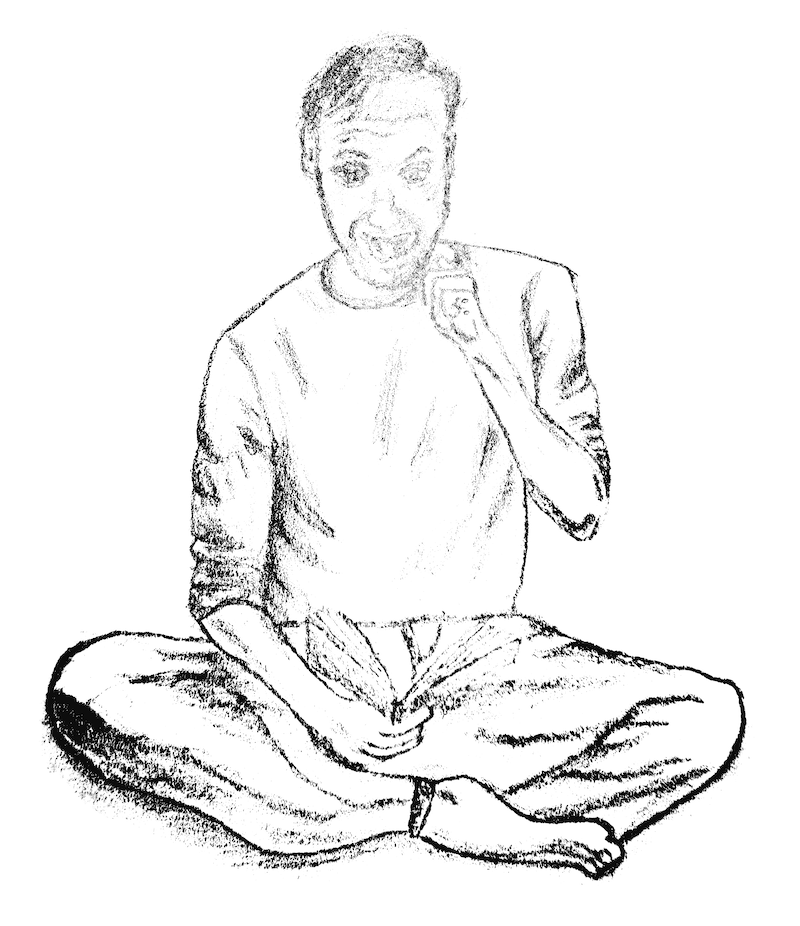
\includegraphics[width=0.3\paperwidth]{images/testpic}}
    \end{center}\label{img:history}
\end{figure}

``\textit{To know who you are today, I need to know your past, and maybe even can predict something about your future.}''
This applies not only to individuals, but as well to humanity as a whole and localized phenomena like the art of CI itself.
By knowing its origins, we can prevent from diverting too far from it, and reach a more profound understanding of why things are the way they are.
And also, of course, to bring in some kind of attitude of honor, paying our respect to the founding fathers -- and mothers.
To bring in some tradition; something our society these days so much lacks and yet is so much in need of -- even though it might not be aware of it.

\section{Founding Parents}\label{sec:founding-parents}

CI was developed in June \textbf{1972} in the US by mainly a man called \textbf{Steve Paxton}, ``the father of CI'' -- see his picture on the right --, who was an American dancer, gymnastics and choreographer and former Aikidoka (someone who practices the Japanese martial art Aikido) who lived in New York City (by that time mainly performing in the Judson Dance Theater).
He was keen to explore and push the boundaries to develop this new practice, some sort of ``art-sport''.

Next to him, it is worth mentioning \textbf{Nancy Stark Smith} -- ``the mother of CI'' --, who is the one still holding CI, as Steve stopped doing CI about 7 years after its invention, intenting to give it to the people.
She continued with another partner and started the Contact Quarterly magazine, a vehicle to share ideas, to hold the theme and practice of CI\@.

\section{Creation}\label{sec:creation}

In spring 1972, Steve Paxton invited a group of 17 students and colleagues, dancers, martial artists, acrobats, gymnasts and athletes, to explore and research the \textbf{extremes of movement and disorientation} -- from standing still to falling, rolling, colliding and jumping in the air -- in a two-week workshop.
While moving with high velocity, running into each other, bumping, trying to survive, and see what the result will be.\footnote{A little bit like what they do at the Large Hadron Collider at CERN: Smashing some particles at each other and be excited about what would happen.}

He wanted the dancers to work with him on the form he was evolving, and at the end of this week of residency, the group presented a performance named ``Contact Improvisation''.
To see for yourself how those first steps looked like, watch this old black-white recording from 1972: \url{https://www.youtube.com/watch?v=9FeSDsmIeHA}

Out of that exploration, a 20-minutes performance piece called ``\textit{Magnesium}'' arose, whereas the first quarter-hour was about jumping and bumping, manipulation and clinging.
Only the last 5 minutes, the so-called ``\gls{smalldance}'' was performed: A form of meditation that is practiced standing, where attention is paid to postural adjustments and micro-weight transfers.
Videos narrated by Steve about that are available, which are very much encouraged to watch, to also see the progression from those impactful years of '72, '75 and '87.

\section{Institutionalization}\label{sec:institutionalization}

At first, around 1975, it was considered to \textbf{trademark} the term Contact Improvisation, but this idea was rejected in favor of establishing a forum for communication, which nowadays is the website of \href{https://contactquarterly.com}{Contact Quarterly} and is still co-edited by Nancy Stark Smith herself.
So it was never \textbf{institutionalized}, nor was the name \textbf{copyright} protected.
Together with \href{http://www.ecite.org}{ECITE} (the European Contact Improvisation Teachers Exchange), those two can be considered the main international forums ensuring the quality and continuation of CI\@.

The decision was very deliberate to not have any form of legal institute or \textbf{certifications}, free of any hierarchy.
Remember that a certificate usually doesn't mean that that person is good, but just that the certification was passed.

The downside of not having an authority verifying the competence of the teachers is, of course, that when the word was spreading, more and more \textbf{injuries} started to happen; that's why: ``\textit{One should never teach what one doesn't know properly}''.

\section{Further Spreading}\label{sec:further-spreading}

A few years after the founding event, the very first ``Country Jam'' was organized in 1979, where about 50 people came together to freely exchange and dance, without any structure.
Neither a workshop, conference nor a seminar.
Just co-created being, dancing and living in flux.
Later on, it was introduced in new avant-garde (experimental artists) dance schools in the US\@.

The members of the founding group scattered across the US and started to teach the practice.
It became smoother, continuous and \textbf{controlled}, yet still avoiding eye and direct hand contact.
Much emphasize was put on the experience of flow, which is more of an aesthetic choice (Nancy Stark Smith), yet the central characteristics preserved.

\textbf{Europe} was presented with CI first 1873 in Italy, and later Steve Paxton and Lisa Nelson regularly went to the UK and Amsterdam (School for New Dance Development) as the transmission belts for CI in the whole of Europe.
Belgium was visited by Paxton since the 1980s, but apart to certain outbreaks of fever in successful jams, it didn't leave any lasting traces among dancers.

As founding people could be considered (next to Steve Paxton): Nancy Stark Smith, Danny Lepkoff, Lisa Nelson, Karen Nelson, Nita Little, Andrew Harwood, and Ray Chung.

For more detailed information, read books like \textit{Sharing the Dance} and others which you can find in the~\nameref{ch:resources} section.

\section{Then and Now}\label{sec:then-and-now}

It was, for sure, very different back then, and that's why sometimes people would also refer to it as ``\textit{Old School Contact}''.
There was a \textbf{high risk} with very high velocity, and it, for sure, looked very amazing -and very scary too.
Good to know, though is, that they trained on \textbf{mats}, especially at the very beginning (see the videos), which would make the impact of falling much less.
After they started to do the same without mats, though, they got -- quite a lot of -- injuries.

In the last few decades, much more emphasis was put on \textbf{flow}, instead on ``explosion'', and also on figuring out the \textbf{least resistant} pathway.
Some people claim that CI lost quite a lot of its characteristics along the way, yet it could be said that it's nice to have both, to be able to choose what you want.
Being able to survive the explosion, and play comfortably in the flow.

Today there are many different \textbf{styles}: more flow, more impactful, acrobatics, dance, acting, \ldots
The differences are mostly based on the uniqueness of the teachers, along with their lineages; but also due to culturally specifics.
Some countries may have simply other ``body orientations'', resulting in a different CI style.

\section{Future}\label{sec:future}

Hopefully, it will keep a \textbf{strong trunk}, meaning: People keep on researching the practice, while still knowing where it comes from, knowing its roots.
We are all welcoming the \textbf{branches}, e.g.\ CI combined with other practices like ``Contact Tango'', ``Contact Beyond Contact'', and so forth, or CI with using substances for \textit{other states of awareness}.
Hoping for -- as the tree is branching -- that the main trunk will stay the main trunk so that there is no need for the distinction between ``I am a CI \textit{purist}'' but that it's possible to simply say: ``I'm doing CI''.
The trunk has been \textbf{stable} for the last 50 years, yet plenty of new branches appeared in the last 20 years; branches which merge different forms together.
It is important that people be aware that those branches and merges are not CI the way it is actually practiced.
And lastly, what's needed are good teachers, jams, and spaces where the ideas and principles are held from CI: Knowing the physical aspect but also keeping the history.

\chapter{Principles}\label{ch:principles}

\chapterCoverImage{principles}

Many different systems --like with sports, dances or martial arts-- are focused around dozens or even hundreds of \textbf{techniques} which are given to the student to learn by hard, including their names, and precise definitions of what's the right way of doing it.
This is an approach which might work for many instances, but obviously has some serious disadvantages when it comes to quickly responding (picking the right technique from many within a split of a second) and more importantly the ability for individual expression (using the system as an art-form to ``say the unsayable'').

In contrast to that, CI --along with many other systems as well-- is centered around a few core principles, and every technique which might be taught, studied and practiced is a manifestation of those core principles and are based upon them.
There are therefore no real moves to be learned, but more principles to be embodied and applied in any given moment, and adjusted to whatever needs are present while staying within the boundaries of the principles of that specific system.
Once they are well understood, you can free yourself from the limitations of specific techniques, and questions like whether something is ``right or wrong'' can be easily answered by asking your understanding.
Yet, as it is with the mastery of any art: Once the principles are fully understood, they can be broken if desired so, as: ``\textit{You can do whatever you want, as long as you know what you are doing.}''

\section{In Short}\label{sec:in-short}

As CI is an improvised partner dance --usually, but not necessarily done with two people/bodies--, it encourages the exploration together with the ground, while staying in constant physical contact.
The dance is supposed to move by itself, according to the participants aims and wishes.

In short, these are the basic principles used in CI, whereas the first two could be considered the physical essential ones and the other more about attitude and technique:

\begin{itemize}
    \item \textbf{Sharing Weight}
    \item \textbf{Rolling Point of Contact}
    \item Exploration of \textbf{Physical Forces}
    \item \textbf{Spirals} (and other related movement patterns)
\end{itemize}

Once all those principles are embodied, they will show up and surprise you when they happen and change your pathways.
They will also very much show up when in high velocity, when going into a risk engaged dance, dancing with a super high level of alertness and attention, jumping on each other, yet landing safely back on the ground.

\section{Grounding}\label{sec:grounding}

With grounding we are referring to some kind of sensation of (light) heaviness in the body, which makes the stance more \textbf{stable}, more robust and thus more connected to the ground.
Imaginary language like ``rooting'', and similar, are often used to describe this internal sensation, with its very realistic impact on the external.
This quality is the beginning of it all, without it, we can't go any further, as without a firm foundation, there is no house we can build upon.
To help to improve our groundedness we can use \textbf{visualizations} (roots growing into the ground), focusing our attention to where the sole of the feet have contact with the floor, breathing out and relaxing the muscular tension without collapsing in one's structure, and simply thinking about words which are associated with a grounded, firm, or stable quality.

It should not be confused with stiffness or rigidity, which so often lead to the illusion of groundedness and is achieved by simply contracting all muscles; something we don't want to do as it will remove the ability to adapt to the moment, remove our flexibility.

Lastly, because of the interconnection between \textbf{body-mind}, the fact that you become a more grounded mover physically, you also become a more grounded person mentally (emotionally stable, more resilient, durable).

\section{Small Dance}\label{sec:small-dance}

Recognizing and listening to the \gls{smalldance} is a starting exercise helping the practitioner to increase his \textbf{body awareness}.
It is usually done standing --and at the beginning, this was the only of doing it--, as it is the strongest way to balance due to the small surface.
Which position to take is not as important as the perception of reaction to the \textbf{process of balance}, which is always happening --except when completely lying down--, in any position.
Ultimately, you want to be able to figure out your own and also your partner's center, as lifts and basically, everything starts happening from there.

It could be considered as a form of \textbf{mindfulness} practice, where we focus our full attention to the sensation of standing; especially of the micro-movements in our ankles and whole body.
The process of how some automatic movements, little contractions and twitches, keeping us standing upright.
Something that is beyond our consciousness, but something we can definitely tap into by being more sensitive to it.
We can also use those unconscious micro-movements as a source of movement by amplifying it.

It is often used as a beginning of a grounding exercise, by shifting the weight, and keeping the center low.
Additionally, once the weight was totally shifted to one side, to ``double ground'' oneself to have an apparent sensation of stability and balance.

\section{Pouring Weight}\label{sec:pouring-weight}

Once we have succeeded to ``gain some weight by grounding'', we can use that to pour it into another person's body.
The emphasis here is to \textbf{slowly and gradually} increase the amount of pressure where the bodies have contact, instead of a quick and sudden shift, which will be difficult and fear evoking movement for your partner; ultimately even dangerous.
Instead, we want to ``announce'' that there is some weight approaching so that our partner can adjust and adapt posture and internal tension/structure to that poured weight.

\section{Sharing Weight}\label{sec:sharing-weight}

The first and most important principle is trying to seek a deep --core-- connection between two bodies, something we call in our classes as an ``\textit{oomph}''-quality.
The body is \textbf{stable and grounded}, yet its limbs and joints are \textbf{soft and relaxed}; \textit{like an iron stick wrapped in cotton wool}.
Also, the contact is primarily on \gls{thebox}, the upper body, and less on the arms and legs.
It is different from actively pushing with muscular force, and also slightly different from leaning, by which you shift your center of gravity beyond a point of no-return.

The contact should lead to a sensation of the \textbf{ground underneath} your partner's feet, passing through their center, originating from the single point of contact which can be even as far from the ground as a hand.
We constantly try to search for the \gls{centergravity} of the other person's body, which might sound familiar to people with a background in martial arts such as Taijiquan.
This is also called a \textit{contact quality}, a result of grounding plus sharing weight, instead of a simple \textit{touch quality}, a soft feather stroking like a butterfly.
The ultimate goal is to maintain this quality throughout (almost) all time, and therefore also leading to acquiring the skill of \textbf{recognizing weight}.

Unfortunately, this is also usually one of the \textbf{most difficult} skills to acquire for beginners.
Reasons could be such as fear of falling, fear of imposing one's own weight on another person, being a burden and thoughts popup like: ``\textit{Am I too much? Am I too heavy for the other person?}''
A handshake or a tap on the shoulder is common in our society, leaning on someone not.
It's important to learn this principle, yet without stopping to breathe and without tensing up, which can be a massive struggle, especially for beginners.
Another very scary aspect for many people is when going to the ground.
Having lots of weight on you or giving (lots of) weight to that person on the ground is something which needs to be trained.
We don't only share our weight, but we are also sharing our balance, in order not to be off-balanced but ``\textbf{shared-balanced}''.

The more advanced you get, the more you have already acquired that skill, the more often you can choose to deliberately not give weight in the right moment.

\section{Rolling Point of Contact}\label{sec:rolling-point-of-contact}

We use spiraling and rotating movement patterns to always \textbf{maintain contact} and amount of pressure in a rolling fashion, instead of sliding or even jumping the point of contact, e.g. directly from a hand to a shoulder, not passing ``through'' the whole arm.
Sliding or jumping (point of contact) is by no means wrong, but it is added later on deliberately by more advanced practitioners.

The contact will thereby follow a \textbf{predictable trajectory}, a pathway, which means both partners can anticipate the very next movement, which furthermore leads to a more ``fluid sensation'' in the dance.
There is no disengaging or re-engaging of the point of contact (at least not at the beginning), which sometimes can feel like little bumps during the dance, breaking this fluid sensation.
For this to happen, it is required to have a more agile body, bulging out body parts and bending/flexing wherever necessary to keep a clear rolling point of contact; something we refer to as an ``octopus''-quality.
It is also used to correct each other to find balance, to readjust and realign.

This is the second most important and also the second most often principle with which beginners struggle with.
Be aware that we don't aim for \textbf{intimate body-parts} (buttocks, breasts, genitals), yet we roll over them ``coincidentally'' without staying there.
For example, when my head would be at those parts, I will still try to avoid that if possible, even if we know each other very well.
We try to desexualize the human body --not the partner, but the body--, something which can be indeed difficult in our hyper-sexualized society.
The touch should be without any sexual intention, even if intimate parts are being rolled over, which will make us both feel comfortable; the ``how'' is more important than the ``what''.
We play with each other, just like kids are playing ``rough and tumble'' in the playground, before encountering the wonderful world of sexuality.
Just like a doctor touching breast tissue intending to find signs of cancer and without any sexual intention or gain some personal advantage; that's why it feels safe for the patient to receive that touch.

\section{Pathway Continuation}\label{sec:pathway-continuation}

To be aligned with the physical law of \textbf{inertia}, we should never break an already moving momentum; exceptions again made for those who have mastered it.
Once spiraling in one direction it should be maintained; it opens up the possibility for anticipation, predictability and therefore trust on a psychological level, but also a mere reason of energy efficiency on the physical level.

\section{Movement Patterns}\label{sec:movement-patterns}

Through a heightened awareness of communication through movement, touch, and sharing weight, we explore the space and the connection between, through mutual physical cooperation.
Fundamental movement patterns are:

\begin{itemize}
    \item [] \textbf{Yielding}: softening/surrendering into incoming force or to gravity
    \item [] \textbf{Pushing}: expansion, taking up space
    \item [] \textbf{Reaching}: extending physically or meta-physically
    \item [] \textbf{Pulling}: contraction, until collapsing
    \item [] \textbf{Releasing}: relaxing into what's contracted before
\end{itemize}

All of those movements can be done easily with little muscular effort if basic physical forces are acknowledged and taken advantage of, such as gravity (falling), momentum, inertia, balancing, etc.
And all of those while staying in contact.

\section{Relaxation}\label{sec:relaxation}

We usually move rather relaxed; a body which is ready for action yet open for receiving tactile stimulus, open for information.
We try to achieve that by deep breathing, by keeping a fluid movement quality (``octopus''-quality) and also avoid a staring eye gaze.

Yet, a relaxed state should not be confused with a collapsed one.
An active state is also not the same as a hyper-tensed one.
Within this spectrum of non-extremes, we ought to find the optimal amount of \textbf{muscle tone} which is appropriate for a given situation.

\chapter{Mottos}\label{ch:mottos}

\chapterCoverImage{mottos}

Mottos are like universal \textbf{guidelines}; like a line that helps us to keep track in case we need it when we are lost.
They are not rules, but there are more like \textbf{invitations}: There will be no consequences once they are not adhered.
And it is up to us to face to them when we need them, and they don't come to us once we disregard them.
They help us improve our technique, implement the principles, and embody a quality more conforming to the core of CI\@.

%You could also call them --universal-- guidelines, which would be semantically more specific than principles, yet not as specific as concrete techniques.
%They are kept short, so we can remember them quickly, and can act as part of our vocabulary.
%Once we mention it to someone who is also familiar with that saying, we immediately have a common understanding within a very short period of time; something that is identical to the benefit of introducing a~\nameref{ch:jargon}.

\newcommand{\motto}[1]{
    \vspace{5pt}
    \begin{adjustwidth}{30pt}{30pt}
        \begin{center}
            \textit{#1}
        \end{center}
    \end{adjustwidth}
}

\motto{Tension masks sensation.}

Image your nerves like little pipes running throughout your whole body.
Now imagine whenever you tense up, your muscles contract which surround those ``nerve pipes''.
By contracting so much, they start to squeeze the nerves so that they can't transmit any information anymore; they are blocked.

The more \textbf{relaxed} we are, the more sensitive our skin is to touch, pressure and weight.
Of course, we want to relax, yet not totally collapse; any extreme is to be avoided.
We want to engage with the minimum effort possible to stay stable; as little as possible, as much as necessary.

\motto{Keep on breathing.}
When getting tensed up, physically and/or emotionally, we usually have the tendency to automatically hold our breath.
This is rather counterproductive for staying sharp, focused and relaxed.
Instead, we continuously try to remind ourselves to breathe.
Especially emphasizing the (deep) out-breath, as the exhalation activates our parasympathetic nervous system.
Do that through your mouth, relaxing the jaw, and don't suppress, but also don't force, to make a sound.

Breathe out when you notice that your partner becomes stiff and holds his breath.
It is an effective way to non-verbally co-regulate your partner into taking a big sigh as well.
It's a little bit like with the phenomena of yawning: Due to our social nature, equipped with mirror neurons, those behaviors tend to be contagious, and we can't help it but imitate it.

\motto{We try not to fall in love with our partner,\\we fall in love with the dance.}
Try to see your partner as a mere physical object and by that explore the physical realm instead of the psychological, the interpersonal one.
It's also not a personal dance, it's a physicality; the experience is because of the practice, not because of your partner necessarily; don't attach that to a specific person, just like the teachings of Tantra tell us as well.
Even when you had a remarkable dance with someone, once the dance is over, I'm going to say ``Thank you, and bye bye''.
It is nevertheless possible, of course, to talk to that person later on, but please don't linger and dance the entire class or jam with that single person.

\motto{Keep eyes open and ``wide''.}
Sometimes people tend to close their eyes, or focus them constantly, fierce-fully on their partner.
Instead, we want to keep an open gaze, perceiving everything around us, staying in connection with all the people in the room and the room itself.
Once we start to gaze at the floor, this is usually an indication of a state of hyper-focus, which potentially closes our perception.
Remind yourself to keep your vision leveled, stay aware and attentive.

\motto{Dance at the edge of your level of attention,\\and don't cross the level of your partner's attention.}
Try to \textbf{expand} what you can do regarding movement, attention, speed, techniques, and pathways.
And also vital, listen to what your partner is able as well, and \textbf{respect} that with patience and compassion.

\section{Inspirational Mistakes}\label{sec:inspirational-mistakes}

As in general with any improvised art, mistakes are only seen as such, as soon as we declare them as being mistakes.

Imagine two improvisation actors on stage.
One says ``mouse'', the other says ``house''.
And then again, the same thing: house, then mouse.
They actually intended to go on with different rhyming words, but for whatever reason (too nervous?) they are stuck and can't come up with something new, and because they can fake it as a deliberate decision (not admitting it being a mistake, something which was not their initial desired goal; when things don't go according to a fixed plan), people in the audience might be amazed by the ``post-modern acting skills'' and interpret something into it which is actually not there.

Once you can let go of any plan, and be truly in the \textbf{present moment} with whatever is happening; once you can fully comprehend that whenever there is another person involved, any desire for control is futile \ldots then you will be able to surrender and use any happening as a source of inspiration.
Ultimately, being able to \textbf{surprise yourself}, and be fascinated by what happened to you once you let go.

\chapter{Techniques}\label{ch:techniques}

\chapterCoverImage{techniques}

Although CI is a \textbf{principle-based system}, meaning it doesn't have a defined set of techniques which are universally taught and practiced, there are certain reoccurring movements (``tricks'') which could be considered as techniques.
Yet, they should not be regarded as something to be followed literally, and as long as you stay within the framework of the CI principles, any adaption can be judged as correct.

\section{Technique or Principle?}\label{sec:technique-or-principle?}

The difference between technique and principle of CI is like the difference between grammar (universal and abstract) and vocabulary (specific and concrete) of language.
Even in the United States we will use the same grammar, but the words/vocabulary, and especially style/dialect will be slightly different from in the United Kingdom, Australia or anywhere else in the world; expect small hiccups to happen.
Nevertheless, we will be able to \textbf{understand} each other as the principles, the grammar stays the same.
And often it will be necessary to stay a few hours with a new teacher to embody his body language, from which the vocabulary comes.
Vocabulary, like lifts, is a rather \textbf{regional expression} of the application of the commonly shared principles.

\section{Lifts}\label{sec:lifts}

The most common -- and most impressive -- ``spice'' added to a dance are lifts.
Whenever one center is located underneath another center, a lift can be easily performed by ``pouring one's weight''\footnote{Pouring weight is one of the core principles of CI, slowly and continuously increasing the pressure, instead of jumping on our partner with a potentially heavy impact and possible injury} onto the base.

There are different kinds of lifts, but the most typical ones are hip and shoulder-lifts.
When performing a \textbf{hip-lift}, the \gls{over-dancer} usually places his butt, lower belly or side on the lower back of the \gls{under-dancer}.
The \textbf{shoulder-lift} is the highest level of a lift where one ``flies'' on the shoulder of the other person.
Those lifts are usually done standing and also while being in the ``little animal'' position, and to change for example from a hip to a shoulder-lift, the over-dancer can spiral upwards the back defying gravity.

As a base, we need to ground ourselves to become more stable (and heavy) by focusing on our \gls{centergravity},
whereas the flyer, on the other hand, tries to make himself light and engage in his \gls{centerleviathan}.

Lifting might lead to potentially dangerous situations, which require us to pay special attention to the following safety rules:

\begin{itemize*}
    \item \textbf{Not grabbing} is a general guideline, using less the hands and more the torso, yet with lifting this becomes especially important; thus no interlocking of the arms or grabbing the limbs of your flying partners.
    \item Always keep a \textbf{hollow back} (a.k.a. ``good gorilla'') to provide a stable support for your partner instead of rounding your back, which make him feel down and freak him out.
    \item Always keep your \textbf{head above ass}, otherwise your partner will most likely react with a fear response because of the danger of sliding down over your head (especially don't combine this with grabbing/interlocking).
\end{itemize*}

Read more about this in the~\nameref{ch:safety} chapter.

\section{Spirals}\label{sec:spirals}

We use a lot of spirally movement patterns in CI and pay special attention to how they are perceived, seen and anticipated in different movements in our own or someone else's body.
Moving in spirals is the perfect way to keep the pathway continuation which adds to a more enjoyable, fluid sensation during the dance.
Spiraling is considered a core movement pattern in CI and there is much more to say and experience about it.

Spirals can be very visibly be done between two body parts by moving from the distal parts of the body towards the more proximal parts.
There is a lot possible with playing with the axis, changing the axis, going within or outside the body, \ldots the limit is the imagination (and skill).
And ultimately spirals can also only by visualized, imagined, with pure intention/attention without any external visibility of movement.

% TODO exercise reference: touch points, connect them with a spiral

\section{Negative Space}\label{sec:negative-space}

Dancing in the so-called \gls{negativespace} basically means entering, usually by reaching into it with a limb, the \gls{kinesphere} of another person without engaging in touch.
This is a common way to non-verbally invite someone for contact, to start a dance together, at a jam for example.

\section{Other Techniques}\label{sec:other-techniques}

\textbf{\Gls{body-surfing}} happens when one person rolls on the floor, and the other (usually) perpendicularly rolls over him.
Watch out if your partner is too heavy, to be able to release/distribute his weight, or simply drop your partner off in a gentle and polite way.
This usually evokes a lot of laughter due to the fun nature of it, its playfulness which reminds us of our childhood games we played.
For even more fun, consider doing a body-surf with more than two people and make some sort of ``body train''.

\textbf{Counter-balancing} is commonly used in partner-acrobatics, where the center is, for once, oppositional, instead of centers being shared.
We basically ``lean away'' from the partner, and by holding on to each other somehow, we balance each other out.

\chapter{Safety}\label{ch:safety}

\chapterCoverImage{safety}

When thinking about safety, we might immediately think about \textbf{physical} safety:
To avoid injuries, disproportional risks, and dangerous situations.
Next to that, we also need to ensure our \textbf{psychological} safety:
The emotions we experience and how they are expressed, and especially when it comes to topics around intimacy and consent.
Lastly, there is also something like \textbf{social} safety: The way we behave and ought to behave; the implicit norms of a subculture, and simple etiquette like dresscode.

\section{Protection}\label{sec:protection}
%%%%%%%%%%%%%%%%%%%%%%%%%%%%%%%%%%%%%%%%%%%%%%%%%%%%%%%%%%%%%%%%%%%%%%%%%%%%%%%%%%%%%%%%%%%%%%%%%%%%%%%%%%%%%%%%%%%%%%%%

Many of us exercise to keep our body \textbf{healthy}.
Yet it sometimes happens that while we are doing so, we injure our body, destroy our health, damage what we initially wanted to protect.
It seems like a terrible contradiction, that the one thing which is supposed to heal, suddenly harms.

That is why safety is of the utmost importance when practicing CI\@.
Just like acrobatics, there are sometimes some more dangerous techniques involved, which require us to pay special attention to this aspect.
Not only the safety of yourself, but we also want to ensure the safety of the \textbf{other people} we are dancing with and the group as a whole.

And of course, we are not only concerned about the physical but also the \textbf{psychological} safety which needs to be addressed.
The complexity of the social construct around behaviors and norms.
How we deal with psychological triggers, overwhelming emotions, and sexual desires.

How can we navigate through all of these areas still staying safe together?
Let's try to answer that.

\section{Is it safe?}\label{sec:is-it-safe?}
%%%%%%%%%%%%%%%%%%%%%%%%%%%%%%%%%%%%%%%%%%%%%%%%%%%%%%%%%%%%%%%%%%%%%%%%%%%%%%%%%%%%%%%%%%%%%%%%%%%%%%%%%%%%%%%%%%%%%%%%

Safety, in obvious terms of ``free of injuries'', should always come first when practicing any potentially risky movement style such as CI\@.
Furthermore, knowing, respecting and adhering to the local, specific \textbf{subcultural norms} will also lead to psychological/emotional safety within the group.
Besides all these concerns about safety, it is safe to say that CI can be practiced by anyone: professionally trained dancers, recreational movers, athletes, dancers of all abilities and ages.

Yet, if you ask yourself whether CI is safe, then the short answer is simple: No.
It can be \textbf{safe enough}, though, which is what we aim for.
It is for sure less safe than Judo or MMA, but more safe than running or pottery.
Furthermore, it is a high-intense form of dancing, and also more risky due to not knowing what your partner is bringing.
Safety just can't be reached in the outside world, meeting each other; neither physically injured nor psychologically in pain.
So that's why it's important to be aware of the existing risks, and at the same time expanding the boundaries of what's possible.

\section{Consent}\label{sec:consent}
%%%%%%%%%%%%%%%%%%%%%%%%%%%%%%%%%%%%%%%%%%%%%%%%%%%%%%%%%%%%%%%%%%%%%%%%%%%%%%%%%%%%%%%%%%%%%%%%%%%%%%%%%%%%%%%%%%%%%%%%

Consent is mainly about being able to express as well as hearing and appropriately responding to a ``yes'' and a ``no'', which are both possibly, and in the context of CI, preferably expressed non-verbally.

Of course, this starts already when engaging in a dance with someone, but is most importantly when it comes to more advanced techniques like lifts.
A ``no'' could be expressed due to lack of experience with and thus trust into each other, fear of being lifted, considering the other person's weight as too heavy, or other reasons.
There are many elegant ways out so that we can hold ourselves responsible for withstanding our \textbf{boundaries} instead of making others accountable for crossing them, ultimately ``self-dis-empowering'' ourselves.

Whenever a gentle hint by movement does not have the desired result, we can of course always cough, or if all of those subtle cues wouldn't work, simply speak and be very explicit about our wishes by saying assertively and gently with a smile: ``No''.

\section{Technical Safety}\label{sec:technical-safety}
%%%%%%%%%%%%%%%%%%%%%%%%%%%%%%%%%%%%%%%%%%%%%%%%%%%%%%%%%%%%%%%%%%%%%%%%%%%%%%%%%%%%%%%%%%%%%%%%%%%%%%%%%%%%%%%%%%%%%%%%

There are many, many things which can lead to severe injuries, especially when being performed by more inexperienced students.
For the sake of simplicity and conciseness though, we will limit the list to a few, the most common ones, here:

\vspace{10pt}

\noindent \textbf{Head above ass}: When lifting a partner, the shoulders must always be higher than the pelvis, as otherwise the person will slide down overhead with all kinds of undesirable consequences.

\vspace{5pt}
\noindent \textbf{Don't grab}: When encompassing the partner's limb, for example, that part of his body will be immovable and thus prevents him from using it as ``landing gear'' when needed, potentially leading to an accident.
It additionally removes the agency of the other person and is considered to be simply rude.
There is a fine line between ``polite manipulation'' by pushing a bit, guiding, and even offering a welcomed structure/base for the other person on the one hand, and a forceful, dominant directness on the other, which as well can be ok with some dance partners, those you already know well, and they consented to it.
To be fully safe though, especially with strangers or in unknown places, refrain from too much manipulation, or also ``pedipulation'', meaning using the feet to change the shape of your partner.

\vspace{5pt}
\noindent \textbf{Don't interlock}: When people perform a back lift and interlock the arms (and God forbid simultaneously lowering the head below the pelvis) and they fall, the flyer might get into a state of panic and tenses up his arms, while the base will fall and not being able to use his arms, thus falling on his face with the weight of the lifted partner.
I leave it up to your own imagination of the consequences of such an event.

\vspace{5pt}
\noindent \textbf{Don't jump}, especially when being lifted as a flyer.
Jumping and other techniques leading to (uncontrolled) collisions was an essential part of old-school CI, yet in today's development more emphasis is being put on safety.
The impact of jumping on a partner can lead to injuries, especially on the spine, that's why we prefer to pour our weight softly on our partner so that he can adjust, shift his weight and readjust his structure.

\vspace{5pt}
\noindent \textbf{Momentum} is debatable, yet if safety has the highest priority, then it should be avoided as it takes away reversibility because there is no control anymore in the movement.

\vspace{10pt}

For any more risky technique, it's always a good idea to have someone \textbf{spotting} you, someone we usually refer to as a ``\gls{guardianangel}'', who is trying to catch if someone falls on the ground, usually more concerned about the head and less about the feet; never grab the feet!
Don't grab, yet stay ready to engage in case something goes wrong and grab them well to make them land as softly as possible.
For the even more extreme techniques, it can be even advisable to have two guardian angels at the same time.

\section{Intimacy}\label{sec:intimacy}
%%%%%%%%%%%%%%%%%%%%%%%%%%%%%%%%%%%%%%%%%%%%%%%%%%%%%%%%%%%%%%%%%%%%%%%%%%%%%%%%%%%%%%%%%%%%%%%%%%%%%%%%%%%%%%%%%%%%%%%%

The psychological aspect of safety usually revolves around the topics of intimacy, sensuality and sexuality and how to set, perceive and respect \textbf{boundaries} of each other.
Take for example, when engaging in floor work or simply using the rolling point of contact over more intimate body parts, people --and especially women-- can quickly feel uncomfortable.
From the outside (imagine people who don't know the practice) this might seem very intimate, but for the more experienced practitioners, it's pure exploration and physics, an innocent and pure way of play.

Not only on the physical level, because of the proximity in touch, but also on the sensual/sexual level, CI can feel frightening for some people at times.
Just remember, this is not a \textbf{tantra practice} or similar, so sensuality is NOT (!) at CI's core; we don't engage in therapeutic energy work, don't activate Kundalini or seek for cuddle puddles.

Sensuality is a wonderful thing, but it is not really appropriate to go into ``melting'' into your partner, falling in love, or even sexuality, and expressing this via caressing touch, cuddles and somewhat ``lustful behavior'' during CI\@.
This border can be crossed at times, as the positive bonding effects of touch can easily lead us to engage into more.
At this moment, it is advised to \textbf{separate}, to ``cool down'' and re-engage with the dance, instead of the partner.
Caressing the skin of another person, to ``cuddle up'' and all of it is great, amazing, and please do more of it, but please refrain from doing so on the CI dance floor.

There is often a partner \textbf{bodywork} exercise at the end of a class/jam; a typical thing dancers would do.
It is meant to be a more technical, medical, or sports massage, rather than a personal, emotional, intimate touch session; don't confuse those.

If sensuality/sexuality still happens, the \textbf{teacher} will usually take that off very fast, or the jam facilitator, if present.
Cuddles, and cuddle puddles, will often happen and are being tolerated most of the time, yet they are not intentional!
If your intention is to engage in cuddles, the group will notice that behavior, and they might not want to dance with you anymore because of that.
There is of course no strict rule about it, no prohibition, and in some jams they totally tolerate it, even few invite it, but mostly it just doesn't happen.

In classes, it happens very, very rarely that certain individuals will look to satisfy their sexual needs by ``rubbing their horny body on someone else's''.
The teacher will usually here as well take care of a safe space for participants, and stop any form of sexual intended or predatory behavior right away, declaring it as a clear ``no-go''.
That's also why people should go first to a class to learn the \textbf{norms and values}, instead of dropping in a jam right away.
At jams, without a supervisor, no one knows how often such behavior might occur; maybe relatively more often?
Most of the time there is an organizer though, which can repeat clear rules and guidelines in an opening circle, minimizing the probability of such non-welcome behavior.
Comparing CI to Ecstatic Dance or Tantric Dance, in CI there are for sure way, way less ``horny people'' showing up, so you should be safe.

\section{Etiquette}\label{sec:etiquette}
%%%%%%%%%%%%%%%%%%%%%%%%%%%%%%%%%%%%%%%%%%%%%%%%%%%%%%%%%%%%%%%%%%%%%%%%%%%%%%%%%%%%%%%%%%%%%%%%%%%%%%%%%%%%%%%%%%%%%%%%

In every subculture, there are certain (social) \textbf{norms and rules} established which are not written down anywhere.
They somehow float in the minds of the people, the ``bigger body'', everyone carrying an incomplete piece in a slightly different variation, \textbf{implicitly} without any for of mentioning it, and sometimes even without being consciously aware of it.
Yet, if they are broken even just once, there will be consequences for such misbehavior executed by the group.

I, personally, find it useful to try to capture those and make them \textbf{explicit}, so we can avoid unintentional misbehavior and establish as much \textbf{harmony} as possible.
Just know, that every scene, maybe even every group around a specific teacher, has their very own set of normative rules, and that's why this list (as with any other attempt to ``list things'') is just a possible set of many.

\begin{itemize}
    \item \textbf{Talking} is considered to be a distraction during CI classes and especially during jams.
    If verbal communication is indeed needed, there is no obligation for total silence, but be mindful whether it is truly necessary in this moment, or whether it is merely some irrelevant chit-chat.
    In any case, try to keep it as short as possible and the volume low, to not distract your fellow practitioners.
    Otherwise, you can always step off the dance floor and speak properly a bit further away if really needed.
    \item Similarly to talking behavior, which disturbs others, please refrain from \textbf{parking} on the dance floor, meaning: Lying on the floor, maybe even with eyes closed, and being unaware of the surroundings and the other people.
    It is not only an annoyance, as it takes a lot of space (and attention), but it also adds another, yet unnecessary risk factor.
    \item The combination of both (talking and parking) among two or more people, also called \textbf{socializing}, is considered a no-go to do on the dance floor, for the reasons mentioned above.
    For that, please use the edges of the room, and if it's a smaller room, go outside, and if that's not available, just practice letting go and stay in the physical, present moment.
    \item \textbf{Stating your name} is just polite when dancing with someone new.
    At least do so at the very end, and also ask for the other person's name.
    It's just a nice way to acknowledge the person, and potentially useful to furthermore create a friendly bond.
    \item Although probably obvious, yet worth mentioning is \textbf{body hygiene}: Wear fresh clothes (and if you get sweaty easily and/or the temperature is high, also bring several shirts), make sure you have no overly intense bad breath (after having eaten a yummy ``Döner Kebab''), and have taken a shower before engaging in such an intimate movement form with other people.
    There is no need to smell like a perfume shop, as too intense scents are also uncomfortable.
    \item \textbf{Starting slowly} will help you to get to know each other, before \textit{rushing into someone's living room}.
    It's like a handshake, to get a glimpse of whom the other person is, where he is regarding skill and experience, personal preferences and pathways, and then take it from there, building it up, gaining trust, and going on an adventure together.
    \item \textbf{Eye gazing} is another wonderful tool to deeply connect with another human being, yet during CI, we refrain from doing so.
    In our world, it is a wonderful tool to scare people away, making them not liking to dance with you anymore.
    Hopefully, your partners will tell you that this is not the way we do it here.
    We use our peripheral vision to see, and usually don't constantly dance front-to-front.
    \item Speaking about front: It is totally fine to \textbf{roll over the front} side of your partner, and there is no need to avoid certain body parts, like breasts, genital area or similar.
    Once we can depersonalize the partner, seeing it as a physical object and letting go of the stories, there is no need to avoid certain body parts, and rather develop a more innocent and reality bound perspective.
    Yet, of course, we do not seek for it, and if possible, and not disturbing the dance and pathways too much, we try not to go directly for those parts.
\end{itemize}

If you participate in a class, there will be more \textbf{guidance}, and it will be easier for you to spot what's ``right and wrong'' behavior; in a \textbf{jam} though it might be a bit more difficult, especially if there is no hosting facilitator.
Take about 10 minutes at the beginning of a jam to sit, simply watch and observe the communal implicit norms.
Every jam is different, yet there is a common set of baseline rules as mentioned already above.

\section{Clothing}\label{sec:clothing}
%%%%%%%%%%%%%%%%%%%%%%%%%%%%%%%%%%%%%%%%%%%%%%%%%%%%%%%%%%%%%%%%%%%%%%%%%%%%%%%%%%%%%%%%%%%%%%%%%%%%%%%%%%%%%%%%%%%%%%%%

Appropriate clothing is found in every setting where a group forms, sometimes for very rational, practical reasons, and sometimes just to establish some kind of esthetical norm to agree to, a so-called \textbf{dress code}.
If severely violated, it can even lead to the fact that people will feel opposed to dancing with you because of inappropriate clothing, and not because of you as a person!

As such, it is recommended to wear \textbf{long pants and long sleeves} to be able to slide on the ground and have enough friction, as well as sweat soaking capabilities.
Refrain from wearing clothes which limit your movements, like firm jeans, and also shirts (or pants) with buttons on them, as rolling on your partner with your full weight might hurt them, and also your pretty shirt might break; also no zippers for similar reasons.
In short: Normal, dancing, movable sports clothes.
And also plenty of them, especially shirts when the weather is warmer; the minority of us enjoy it to have a partner who is soaked in sweat and dance close with them.

In CI, we need some friction for \textbf{grip}, and for that matter, plastic fabrics will slide more (too much), and thus cotton is better.
Your beloved Adidas pants are not advised as they are too slippery; sorry.
Speaking of grip: It's better to dance \textbf{barefoot}, without socks to avoid slipping, or socks with those plastic nobs on the bottom if you got some of those.

The single utility though which could be useful would be knee pads, as there might be plenty of floor work and carrying people on your body while in the table-top position.
They shouldn't restrict your movement, so preferably choose some which are a bit thinner and made from an elastic material.

Obviously, \textbf{jewelry}, like big earrings, bracelets, rings, and basically any form of it, is not advised as they can get trapped on the other person's body and clothes, ultimately hurting someone.

Ultimately, we don't dress to impress, but rather prefer to wear our \textbf{cozy pyjamas}.
Newcomers often stand out at the beginning wearing overly sexual clothes, showing a lot of skin, or wearing their gym clothes.
All of it which isn't wrong by itself, not at all, it just might not be the right place for it.
You wouldn't wear your favorite onesie pyjama at your mother's funeral, either, would you?!

\chapter{Jargon}\label{ch:jargon}

\chapterCoverImage{jargon}

There are no universally acknowledged names for techniques, movement qualities, exercises, and so forth, but different teachers try to invent, share, and give credits to their inventions.
Over the time, an \textbf{oral tradition} has been established of passing information.
The following chapter is a rather class specific one, as the language and images developed in the area ``I grew up in'' are very local and not universal at all.
Yet, they might inspire others, or at least provide some humorist, personal benefit for you while reading it.

Introduction of a jargon, using technical, domain-specific terms, is useful to express an idea, as otherwise many, many sentences would be needed whereas instead a single word can suffice as well.
The whole purpose of introducing and using jargon is not to smart-ass, to show off one's own superiority, an act of ego arrogance, or to exclude others by using an exclusive language, but for an increased information exchange and increase in information \textbf{density and precision}.

\section{General}\label{sec:general}

\begin{itemize}
    \item [] \textbf{\Gls{smalldance}} -- The subtle, unconscious micro movements of the body trying to maintain its balance.
    \item [] \textbf{\Gls{kinesphere}} -- The space which can be reached by the body/limbs without taking a step.
    \item [] \ldots \textit{for further general terms, see the glossary at the end of this book} \ldots
\end{itemize}

\section{Onomatopoeia}\label{sec:onomatopoeia}

Sometimes, concepts are just much too fuzzy to be properly put into definite words.
Or there might have just no proper words yet been established, which made it necessary to develop our own few words, or even better: ``sound-terms'' (or onomatopoeia\footnote{Onomatopoeia, which has its Greek roots with the meaning of ``name-making'', which is the formation or use of words such as ``buzz'' or ``murmur'' that imitate the sounds associated with the objects or actions they refer to.}) to convey a certain meaning, quality, fuzzy principle or some abstract phenomena closer to what it meant to be:

\begin{itemize}
    \item \textbf{Botsen}: A conflict which arises when the teacher's instructions lead to a resistance based on an ``internal wisdom''; when the ``inner teacher'' and the ``outer teacher'' clash, we usually opt for the inner one and trust our gut feeling; e.g.\ Being told to jump and do a roll, but it doesn't feel safe and fear/resistance comes up, so you simply don't do it.
    (actually a Dutch word, meaning to clash, to collide; ``bot'' Dutch for bone; like two fists smashed on each other)
    \item \textbf{Hoopedy Di Poop}: Techniques which look overly impressive (good to show-off), yet not necessarily show much skill though, like jumping on each other; e.g.\ fancy technical, acrobatic stuff which usually comes with a higher risk for injury.
    \item \textbf{La La Land\footnote{Yes, ``La La Land'' is also the title of a US musical romantic comedy-drama movie from 2016 with Ryan Gosling and Emma Stone.}}: Referring to anything which is more commonly used in the area of spirituality/religion, metaphysics, esoteric, new age talk and superstitions.
    Yet, sometimes we are still using concepts from those domains nevertheless due to the lack of any other better alternatives; e.g.\ think about when talking about ``reaching beyond the physical body'', which is of course technically not possible, but it gives the right image and intention.
    \item \textbf{Mooshy Mooshy}: (pronounced ``muschi muschi'') Indicating that during a dance, a too sensual, and thus inappropriate atmosphere arises, with no clear intentions; ranging from simply moving very slowly caressing down to \textit{cuddle puddles} where several people like cuddling on the ground.
    This can especially often be observed when starting with dancing on the ground, often preceded by a body-scan, where things can even end up in a sort of pile of bodies (hopefully not as much as in the movie ``The Perfume'' in the end).
    \item \textbf{Oomph}: (pronounced ``umpf'') The preferred quality of contact between two bodies which is characterized by properly giving/sharing weight, creating a sensation of considerable amount of pressure, opposed to only slight touch; feeling each other's groundedness.
    \item \textbf{Weee}: A scream/sung sound usually expressed in moments of heightened levels of alertness/fear, to down-regulate one's own nervous system, counteracting fear/panic, and allowing the body/atmosphere to relax, release tension, and calm down; also to simply express joy about a movement, making everyone smile; e.g.\ when performing more risky lifts.
\end{itemize}

\section{Animals}\label{sec:animals}

Calling things by animal names is beneficial as they have a very visual characteristic, conveying a visceral experience, because of the qualities we associate with those animal.
We mostly use their names to refer to positions, techniques and ``qualities of body''.

% TODO good gorilla
\begin{itemize}
    \item \textbf{Bear}: Similar to the koala, but while sitting on the ground, and the bear hugging around the torso of his partner.
    \item \textbf{Banana}: Not really an animal, but anyway a useful metaphor where the arms and legs are stretched out long, shaping the whole body like a banana; it can be practiced on the ground (a way of movement on the ground, rolling sideways and only the core touching the floor), but applied often while being on the back of a partner to spiral upwards.
    \item \textbf{Chicken Wing}: Using a ``semi lock'' with the arm pit on the partner while being lifted, or similar; often necessary if the centers are not properly stacked and becoming unbalanced.
    \item \textbf{Chicken Leg}: Same as the chicken wing, but with the hip being flexed instead the elbow.
    \item \textbf{Crab}: The opposite of the octopus movement quality: Rigid, sharp, direct, and staccato.
    Think of the exoskeleton of the crab, when it walks sideways with its stiff limbs.
    \item \textbf{Koala}: When being lifted (or better: jumping on the partner's shoulder) hugging the upper body of the partner sideways and thus being very close to his center, while locking with your arms and legs; either around shoulders (more common) or pelvis (less common).
    It can be used as a preliminary technique for a shoulder lift.
    \item \textbf{(Little) Elephant}: Although we do like elephants, we don't like them in our studio, as their name is used to refer to steps/walking, or landing of the feet, which make a loud sound, indicating that there was no control and/or too much stiffness.
    Landing softly with no sound indicates control of movement, reversibility, precision and awareness, and also is a strong indicator of degree of safety with a partner.
    \item \textbf{Little Monkey}: As a little animal (a.k.a.: ``table-top'') but with knees lifted (a.k.a.: ``bear position'') with a light and fluent walking movement.
    Whenever we land silently, it is done so with control and elegance, which ultimately can prevent (serious) injuries.
    \item \textbf{Little Animal}: A table-top position on all fours, yet emphasizing a more dynamic, alive quality than a regular, wooden table.
    Also, when the painter is performing some movements, the little animal is actively supporting him by shaping his back accordingly, tilting and turning, flexing and extending.
    \item \textbf{Panda}: Similar to koala (and bear), but a more specific way of hugging, with belly to belly; often used while on the ground lying, keeping the centers connected all the time.
    \item \textbf{Snake}: Similar to octopus, but with a slightly different image to connect differently; having many movements in hands and spine going on simultaneously.
    \item \textbf{Octopus}: A movement quality which indicates aliveness/relaxation in all joints/body parts, each of them being controlled by their own intelligence; fluid, soft and smooth; opposite of the crab.
\end{itemize}

\chapter{Movement}\label{ch:movement}

\chapterCoverImage{movement}

We will take a look at the fascinating science of movement, movement theory and a bit of biomechanics, and also deal with more abstract views on movement as maybe known from the dancing world.
For more experienced (improvisation) dancers, a lot of the things mentioned here might sound familiar.
For the more inexperienced among us, this can open a totally new perspective on movement.

\section{Movement Qualities}\label{sec:movement-qualities}

There are different imagined \textbf{dimensions} we can play with, to tap into different qualities on how to use our body, giving it a different flavor, allowing us to do different techniques, and by knowing the pros and cons of each quality, we can apply them in the right moment to elevate our technical skill and also keep things safe for ourselves and our partner.

\subsection{Movement Patterns}\label{subsec:movement-patterns}
%%%%%%%%%%%%%%%%%%%%%%%%%%%%%%%%%%%%%%%%%%%%%%%%%%%%%%%%%%%%%%%%%%%%%%%%%%%%%%%%%%%%%%%%%%%%%%%%%%%%%%%%%%%%%%%%%%%%%%%%

Through a heightened awareness of communication through movement, touch, and sharing weight, we explore the space and the connection between, through mutual physical cooperation.
Fundamental movement patterns are:

\begin{itemize}
    \setlength\itemsep{0em}
    \item [] \textbf{Yielding}: softening/surrendering into incoming force or to gravity
    \item [] \textbf{Pushing}: expansion, taking up space
    \item [] \textbf{Reaching}: extending physically or meta-physically
    \item [] \textbf{Pulling}: contraction, until collapsing
    \item [] \textbf{Releasing}: relaxing into what's contracted before
\end{itemize}

All of those movements can be done easily with little muscular effort if basic physical forces are acknowledged and taken advantage of, such as gravity (falling), momentum, inertia, balancing, etc.
And all of those while staying in contact.

\subsection{Muscle Tone}\label{subsec:muscle-tone}
%%%%%%%%%%%%%%%%%%%%%%%%%%%%%%%%%%%%%%%%%%%%%%%%%%%%%%%%%%%%%%%%%%%%%%%%%%%%%%%%%%%%%%%%%%%%%%%%%%%%%%%%%%%%%%%%%%%%%%%%

We can play a lot with tone, which is the amount of tension we create in our muscles that makes us either more relaxed or more stiff.
In general, we prefer to maintain the least amount of effort, a minimum muscle tension; as little as possible, as much as necessary.
By being more relaxed, we are more flexible, can adapt to an ever-changing situation, and also are more receptive via our tactile sense, being able to receive more information, to listen better.
To have some images to play with, think of moving through air (well, you don't have to imagine that, as we constantly do that --duh).
Instead, think of you being a cloud, floating through the sky (sure, that's better, we usually never do that one).
Now increase tension by imagining moving through water, how it creates a small but continuous resistance, preventing you from sharp, edgy movements, from breaking a fluent pathway.
The next increase in resistance could be achieved by imagining something like honey, sticky and slowing down your movements, having you to add more muscle effort.
And as a final step, imagine being stuck in concrete, which maybe has not yet fully harden, still making you almost unmovable.

\subsubsection{Relaxation}

We usually move rather relaxed; a body which is ready for action yet open for receiving tactile stimulus, open for information.
We try to achieve that by deep breathing, by keeping a fluid movement quality (``octopus''-quality) and also avoid a staring eye gaze.

Yet, a relaxed state should not be confused with a collapsed one.
An active state is also not the same as a hyper-tensed one.
Within this spectrum of non-extremes, we ought to find the optimal amount of \textbf{muscle tone} which is appropriate for a given situation.


\subsection{Speed}\label{subsec:speed}
%%%%%%%%%%%%%%%%%%%%%%%%%%%%%%%%%%%%%%%%%%%%%%%%%%%%%%%%%%%%%%%%%%%%%%%%%%%%%%%%%%%%%%%%%%%%%%%%%%%%%%%%%%%%%%%%%%%%%%%%

Moving on to the very obvious dimension of slowness and fastness.
The slow can be extremely slow, to gain lots of information of internal sensations.
The fast can be released in an explosive manner, like a shockwave through the whole body.
Both, and everything in-between, can be alternated rapidly, to gain more control (of speed).

\subsection{Kinesphere}\label{subsec:kinesphere}
%%%%%%%%%%%%%%%%%%%%%%%%%%%%%%%%%%%%%%%%%%%%%%%%%%%%%%%%%%%%%%%%%%%%%%%%%%%%%%%%%%%%%%%%%%%%%%%%%%%%%%%%%%%%%%%%%%%%%%%%

The degree of extension of the limbs into the space --without stepping-- is called \gls{kinesphere} with which we can play with.
We could segregate it into a small (body), medium (elbows, knees), large (wrists, ankles) and extra large (fingers, toes), and something more abstract going even beyond (projecting outwards), the universe.
Each of them is creating a differently sized ball, or more like an egg shape, around us in which we are limited to move within and also want to stay in constant contact with.

\subsection{Levels}\label{subsec:levels}
%%%%%%%%%%%%%%%%%%%%%%%%%%%%%%%%%%%%%%%%%%%%%%%%%%%%%%%%%%%%%%%%%%%%%%%%%%%%%%%%%%%%%%%%%%%%%%%%%%%%%%%%%%%%%%%%%%%%%%%%

Next to extension into space, we can, of course, take different levels in vertical space: Up (standing), middle (hinged, or on hands and knees being a ``little animal'') and floor work (lying on the ground).
With the help of relaxation and tension, we can quickly change our position on the vertical axis and play with explosive dynamics.
Also, mirroring your dance partner, staying at a different (not the same as with imitating) level then he, can be an challenging, fun, and engaging experience to explore.

\subsection{Isolation}\label{subsec:isolation}
%%%%%%%%%%%%%%%%%%%%%%%%%%%%%%%%%%%%%%%%%%%%%%%%%%%%%%%%%%%%%%%%%%%%%%%%%%%%%%%%%%%%%%%%%%%%%%%%%%%%%%%%%%%%%%%%%%%%%%%%

The isolation of certain body parts can also be fun --and challenging at the same time-- to play with.
The most simple one is to divide the body into upper and lower, left and right side, same side or cross side (homo- or contra-lateral, see the anatomy section for explanation of terminology), or move only in a certain plane.

\subsection{Shapes}\label{subsec:shapes}
%%%%%%%%%%%%%%%%%%%%%%%%%%%%%%%%%%%%%%%%%%%%%%%%%%%%%%%%%%%%%%%%%%%%%%%%%%%%%%%%%%%%%%%%%%%%%%%%%%%%%%%%%%%%%%%%%%%%%%%%

The forms we are drawing in air can be another dimension.
Think of straight lines (edgy, staccato) versus roundness (flowy, fluid, air).
People who have experience with the practice of 5 Rhythms might be familiar with those concepts and make use of them.

\subsection{Combination}\label{subsec:combination}
%%%%%%%%%%%%%%%%%%%%%%%%%%%%%%%%%%%%%%%%%%%%%%%%%%%%%%%%%%%%%%%%%%%%%%%%%%%%%%%%%%%%%%%%%%%%%%%%%%%%%%%%%%%%%%%%%%%%%%%%

To bring those qualities to a next level, try to \textbf{combine} them in different ways.
Often slow, fluid and soft go together, but how about changing one of them to the other extreme?!
Or the legs are in the large kinesphere being soft and staccato, while the arms in the small kinesphere and hard and fluid.
Have a partner telling you what parts should be in which quality, to surprise yourself by finding combinations you would not have thought of alone.

\section{Body Awareness}\label{sec:body-awareness}

Let's have a look of how we actually become aware of our bodies.
The biological and physiological base of how this fascinating organic machinery --roughly-- works.

\subsection{Vestibular System}\label{subsec:vestibular-system}
%%%%%%%%%%%%%%%%%%%%%%%%%%%%%%%%%%%%%%%%%%%%%%%%%%%%%%%%%%%%%%%%%%%%%%%%%%%%%%%%%%%%%%%%%%%%%%%%%%%%%%%%%%%%%%%%%%%%%%%%

This is our sense of \textbf{balance} and spatial orientation for the purpose of movement coordination, and is all well known to us.
It consists of two components: The (three, as there are three dimensions) \textit{semicircular canals} for rotational movements, and the \textit{otoliths} for linear accelerations.
Signals from those are sent to the muscles to keep us upright and control posture, allowing us to maintain our desired position in space.
Together with our proprioception, we can understand our body's dynamics and kinematics in any given moment.

\subsection{Proprioception}\label{subsec:proprioception}
%%%%%%%%%%%%%%%%%%%%%%%%%%%%%%%%%%%%%%%%%%%%%%%%%%%%%%%%%%%%%%%%%%%%%%%%%%%%%%%%%%%%%%%%%%%%%%%%%%%%%%%%%%%%%%%%%%%%%%%%

\Gls{proprioception} allows us --as a sort of 6th sense, the ``kinesthetic sense''-- to be consciously aware of movement, force and body \textbf{position}.
It tells us our body's position in the space, that is the relative positioning of neighboring body parts, and the strength of effort needed for movement.
Try for example to close your eyes and touch your nose; you will be able to do this without looking (in a mirror, or in complete darkness) because of little cells (little \textit{spindles} which are spring-like protein molecules which are stretched inside your muscles) in your body being aware of the \textbf{amount of stretch} they experience (joint position sense), which is then processed subconsciously by your brain giving raise to a bodily sensation.
Everyone is familiar with the knee-jerk reflex, where the patellar tendon is rapidly stretched to an extreme (usually with the help of a hammer), which leads to an immediate response (a reflex) to counteract that and protect the tissue from injury.

Related sensations are \textit{exteroception}, the perception of the outside world, and \textit{interoception}, the perception of internal sensations like pain and hunger.

\subsection{Kinesthesia}\label{subsec:kinesthesia}
%%%%%%%%%%%%%%%%%%%%%%%%%%%%%%%%%%%%%%%%%%%%%%%%%%%%%%%%%%%%%%%%%%%%%%%%%%%%%%%%%%%%%%%%%%%%%%%%%%%%%%%%%%%%%%%%%%%%%%%%

\Gls{kinesthesia} is the awareness of position and \textbf{movement} of body parts using sensory organs (proprioceptors, mechanosensory neurons) in muscles, tendons and joints.
It's crucial in muscle memory and hand-eye coordination.
Sometimes it's confused with proprioception, but those two are different concepts.
If you have an inner ear infection for example, and the sense of balance is affected, this would degrade the proprioceptive, but not the kinesthetic sense.
Moreover, proprioception is more about joint position (more subconscious cognitive awareness of your body in space and balance) whereas kinesthesia is more about awareness of joint movement (more conscious body's motion, behavioral).

\subsection{Neuronal Processing}\label{subsec:neuronal-processing}
%%%%%%%%%%%%%%%%%%%%%%%%%%%%%%%%%%%%%%%%%%%%%%%%%%%%%%%%%%%%%%%%%%%%%%%%%%%%%%%%%%%%%%%%%%%%%%%%%%%%%%%%%%%%%%%%%%%%%%%%

\textbf{Neuromuscular control} is the efferent (signal from the central nervous system to the body) response to an afferent (sensory) input, which is the functional component to movement and athletic activities that is referred to as dynamic stability.
Sensory input comes as (different types of\footnote{The four mechanoreceptors are: Meissner corpuscle for heavy pressure, Pacinian corpuscle for vibraiton, Merkel disks for light touch and Ruffini endings for skin stretch}) \textbf{mechanoreceptors} located in muscles, capsules and ligaments, allowing us awareness of joint position, movement, and acceleration.

All that information (vestibular, proprioceptive, kinesthetic) including the visual input is sent to the brain, where it is processed and integrated to allow us to create an overall representation of body position, movement and acceleration.

\section{Notation}\label{sec:notation}

\subsection{Space Harmony}\label{subsec:space-harmony}
%%%%%%%%%%%%%%%%%%%%%%%%%%%%%%%%%%%%%%%%%%%%%%%%%%%%%%%%%%%%%%%%%%%%%%%%%%%%%%%%%%%%%%%%%%%%%%%%%%%%%%%%%%%%%%%%%%%%%%%%

This movement theory --and practice, also called \textit{Choreutics}-- was developed by the Austrian-Hungarian dancer and choreographer Rudolf Laban, to study the natural sequences of movements we follow in daily life; studying ``the art of movement'' to recognize spatial patterns.

When dancing, the term \textbf{\gls{kinesphere}} is used to refer to the space immediately reachable by your limbs without changing your place on the ground.
We can use up a lot of that space within this sphere (\textit{Far Reach Kinesphere}), just a bit (\textit{Near Reach Kinesphere}) or something in-between (\textit{Mid Reach Kinesphere}).

Furthermore, Mister Laban believed that there are three types of movers which prefer different \textbf{levels}: Those who enjoy leaping and springing off the ground move in \textit{High Level}, those with more sensuous movement enjoying the \textit{Central (Middle) Level}, and those who prefer more earth-bound movements who stayed in the \textit{Deep (Low) Level}.

Within the kinesphere we can move from one point to another through different approaches, so-called \textbf{pathways}: When movement is initiated from (or passes through) the body's center we take the \textit{Central Pathway}, along the outer limits of the kinesphere it takes a \textit{Peripheral Pathway}, and when the movement passes between center and periphery it takes a \textit{Transverse Pathway}.

There is of course much more to say about this, including the Laban Movement Analysis (LMA) which is a method and language for describing, visualizing, interpreting, and documenting movement, but this would go beyond the purpose of this book.


\chapter{Anatomy}\label{ch:anatomy}
% TODO maybe rename it, as it is more than that: "biology"
\chapterCoverImage{anatomy}

As with every practice dealing with the human body, a basic understanding of the human anatomy gives a tremendous advantage.
It will allow you to see and \textbf{experience} things differently, knowing about how your body is ``composed''.
The field is, of course, huge, thus it won't be necessary to go too much into details and focus on certain areas.
Yet an understanding of basic terminology is required to be able to \textbf{communicate} in this field.

\section{Terminology}\label{sec:terminology}

The wording used in anatomy/medicine is built from sub-elements (which usually originated from Latin), thus:
Learning first the elements, and then putting them together to be able to infer the meaning of more complex, compound terms.

\subsection{Orientation}

Because a person can stand, sit, lie, or be in all kinds of positions, it is necessary to have an absolute frame of reference to provide orientation instructions.
When someone uses simple language like ``up'' or ``front'', it is not entirely clear what is actually meant, thus the following anatomical terms lead to a more \textbf{non-ambiguous language}.

\begin{itemize*}
    \item \textbf{Anterior/posterior}: front/back
    \item \textbf{Ventral/dorsal}: front/back of the torso
    \item \textbf{Superior/inferior}: above/below
    \item \textbf{Cranial/caudal}: head-/tail-wards
    \item \textbf{Proximal/distal}: towards to/away from center
    \item \textbf{Medial/lateral}: towards/away from the midline
    \item \textbf{Superficial/profound}: more outside/inside the body
\end{itemize*}

\subsection{Movements}

Each body part can move in certain ways and directions based on the type of joint (see below) and how muscles pull on it.
Again, instructing someone to ``move up'' is ambiguous, whereas ``flex the right knee'' is clear as it can be.

\begin{itemize*}
    \item \textbf{Extension/flexion}: increase / decrease joint angle (stretch / bend)
    \item \textbf{Internal/external (medial/lateral) rotation}: rotating the arm / leg counter- / clockwise towards to / away from the body
    \item \textbf{Adduction/abduction}: moving towards / away from the midline
    \item \textbf{Elevation/depression}: moving the shoulder up / down
    \item \textbf{Pronation/supination}: forearm rotation palm facing up / down
    \item \textbf{Dorsi-/plantar-flexion}: move the ankle towards the dorsum (superior surface, up) or plantar (sole, down) also often called ``point''
    \item \textbf{In-/eversion}: sole towards / away from the median plane
    \item \textbf{Opposition/reposition}: thumb and little finger together / spread
    \item \textbf{Pro-/retraction}: anterolateral / posteromedial movement of the scapula (move shoulder forward/backward)
    \item \textbf{Circumduction}: conical (not really circular) movement of a limb extending from the joint it's moved by
\end{itemize*}

If we take for example a simple shoulder roll, it can be dissected in four movements: elevation, retraction, depression, and protraction.
Or similar with drawing circles with the toes, moving the ankle: dorsi-flexion, eversion, plantar-flexion, and inversion.

Terms derived from lateral movement include:

\begin{itemize*}
    \item \textbf{Uni-lateral}: ``\textit{unus}'' meaning ``one'', on one side of the body
    \item \textbf{Bi-lateral}: ``\textit{bis}'' meaning ``twice'', on both sides of the body
    \item \textbf{Homo-(Ipsi-)lateral}: ``\textit{ipse}'' meaning ``same''
    \item \textbf{Contra-lateral}: ``\text{contra}'' meaning ``against'', e.g. arm on one side, and leg on the other side, creating a diagonal, like we do while walking; also one hemisphere of the brain is controlling the other side of the body
\end{itemize*}

Sometimes the Latin word for left (``sinister'') and right (``dexter'') are being used instead.
Check the next time you have a medical report available, like an X-ray, and you will see these terms pop up; consider yourself a nerd from now on.

\section{Structures}\label{sec:structures}

Next to being familiar with the very basic words of positions and directions, we also need to be able to refer to concrete structures (bones and muscles).
Make yourself thus familiar with some (by far not all) anatomical terms, which help you further understand this medical jargon.

\subsection{Bones}\label{subsec:bones}

The human body has \textbf{206 bones} we can (usually) enumerate; yet by birth we have a few more, up to 280.
The head and trunk (the axial skeleton) make up 80 bones and the limbs (the appendicular skeleton) the other 126.
There are 27 bones for each hand (19 for phalanges plus metacarpals, and 8 carpals), and 26 for each foot (phalanges, metatarsals, and tarsals).

\begin{itemize*}
    \item \textbf{Atlas and axis}: two top most cervical vertebrae
    \item \textbf{Clavicle}: the collar bone connecting sternum and shoulder
    \item \textbf{Coccyx}: the tailbone; the last part of the spine
    \item \textbf{Cranium}: the skull (cervical = neck)
    \item \textbf{Patella}: the knee cap (olecranon is the elbow)
    \item \textbf{Processus}: a bulged out structure; usually tendons attach to it
    \item \textbf{Scapula}: the shoulder blade
    \item \textbf{Sacrum}: big triangular bone at the base of the spine
    \item \textbf{SIAS}: Prominent hip bone (Spina Illiaca Anterior Superior)
    \item \textbf{Vertebra}: An irregular bone forming the spine / vertebral column.
    \item \textbf{Sternum}: the chest bone
\end{itemize*}

For the sake of completeness, it is mentioned that we have true ribs (1-7, sternum connection), false ribs (8-10/12, cartilage), and floating ribs (11-12, no connection).
Also, the spine consists of 33 vertebra: 7 cervical, 12 thoracic, 5 lumbar, 5 fused sacral, and 4 fused forming the coccyx.

\subsection{Muscles}\label{subsec:muscles}

There are \textbf{between 600 and 840 muscles} within the typical human body, depending on how they are counted, and some variations due to mutations.

\begin{itemize*}
    \item \textbf{Abs}: abdominal muscles with 3 layers wrapped around the belly
    \item \textbf{Core muscles}: everything attached to the spine; not only the abs
    \item \textbf{Diaphragm}: muscle for breathing at the bottom of the ribs
    \item \textbf{Glutes}: buttocks consisting of maximus, medius, et minimus
    \item \textbf{Obliques}: part of the core, at the sides of the abs
    \item \textbf{Pectoralis}: the chest muscle (major and minor)
    \item \textbf{Pelvic floor}: similar to diaphragm but at the bottom of the torso
    \item ``\textbf{Stomach muscles}'': the stomach is an organ, which indeed has (involuntary) muscles, but it's located on the left side underneath the ribs, and should not be confused with the abs / lower belly!
    \item \textbf{Trapezius}: at top shoulder around the neck
    \item \textbf{Transverse}: part of the core, like a belt around it
\end{itemize*}

\section{Planes}\label{sec:planes}

\begin{wrapfigure}{R}{0.3\textwidth}
    \centering
    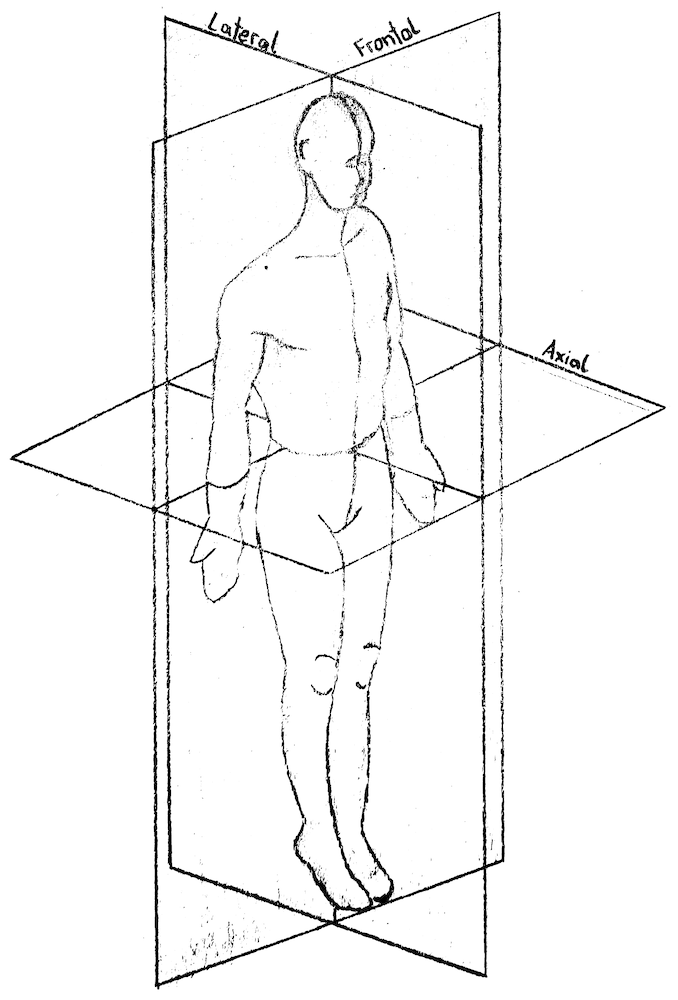
\includegraphics[width=0.3\textwidth]{images/anatomy/planes}
    \caption{The three anatomic \textbf{planes} for the human body.}
\end{wrapfigure}

We differentiate 3 different anatomical planes in which movement can happen:

\noindent \textbf{Frontal Plane}: Also called \textit{Coronal Plane} or \textit{Vertical Plane} and, not surprisingly, represents the plane when looking from the front of the body, dividing the body into an anterior/posterior part.
The directions can be medial/lateral, thus resulting in the movements of ad-/abduction, elevation/depression and in-/eversion.

\noindent \textbf{Lateral Plane}: Also called \textit{Sagittal Plane}, \textit{Longitudinal Plane} or \textit{Anteroposterior Plane}, which is going through the midline and shows the body when looking from the side, separating it into a left/right part.
The directions are thus anterior/posterior and movements are flexion/extension and pro-/retraction.

\noindent \textbf{Axial Plane}: Also called \textit{Transverse Plane}, \textit{Horizontal Plane} (the other two planes are vertical) or \textit{Cross-Sectional Plane}, and divides the body into a top/bottom part.
Directions are thus superior/inferior and allowing movements like rotation, supination/pronation and circumduction.

\section{Joints}\label{sec:joints}

Bones are connected through joints where muscles (together with tendons) can evoke movement.
For different movements, \textbf{different types} of (synovial) joints are needed:

\begin{itemize*}
    \item \textbf{Ball/Socket}: free movement; e.g. hip, shoulder
    \item \textbf{Pivot}: rotation; head (atlantoaxial), elbow (radioulnar)
    \item \textbf{Hinge}: flexion/extension; elbow (humeroulnar), knee
    \item \textbf{Saddle}: fingers-hand (trapeziometacarpal)
    \item \textbf{Condyloid}: fingers/wrist (metacarpophalangeal)
    \item \textbf{Plane}: hand (intercarpal) and feet (tarsal)
    \item \textbf{Gliding}: mini bones in feet
\end{itemize*}

\chapter{Physics}\label{ch:physics}

\chapterCoverImage{physics}

Physics is a huge and fascinating science, dealing with the big (astronomy, astrophysics), the small (nuclear and particle physics), the universal (electromagnetism, thermodynamics) and the more complicated (quantum physics, relativity); basically how the universe behaves, or at least how matter moves through space and time as well as energy and force.

For our purpose though, we will focus on \textbf{classical physics}, mechanics to be precise and its sub-branches, the fundamental concepts of time, space and how they give rise to higher phenomena encountered during CI, and we won't go into the realm of quantum physics as this is beyond the human perception and not of any use to us.
An understanding of physics isn't really needed though --to use it, to play with it-- as it doesn't actually help on a perceptual/experiential, bodily level.

In CI, we engage in the exploration of physics, to play with physical forces, with the direction of movement and its changes in space.
It might be interesting though to see what you learned in physics, to see what's yet \textbf{embodied}.
Engineers might smile hearing terminology from the world of leverage, friction, mutual point of contact, center of mass and so on.
Preferably, after that chapter you are also familiar with terms such as gravity, vector, inertia, force, momentum, and kinetics.

\section{Energy}\label{sec:energy}

The word ``energy'' is just too often misused in the spiritual world as some metaphysical, psycho-telepathic \textbf{mystery}.
In physics, we define it simply as ``\textit{the capacity for doing work}'', and as such different forms exist: potential (position), kinetic (movement), thermal (heat), nuclear (atom), electrical (charges), chemical, and so on.
All forms of energy are associated with motion: Any given body has kinetic energy if it's in motion.
A tensioned device such as a bow, a spring, or your tendons, though at rest, have the potential for creating motion; it contains potential energy.
Energy can neither be created nor destroyed, but only transformed from one form to another, which is stated in the first law of thermodynamics: energy conservation.

\section{Mechanics}\label{sec:mechanics}

Here we are interested in the relationship between force, matter and motion, as seen from a Newtonian perspective, focusing on motion (\textbf{kinematics} or ``\textit{the geometry of motion}'') and forces (\textbf{dynamics}).

Newton's laws of motion (classical mechanics) state:

\begin{enumerate}
    \item ``\textit{A body remains at rest, or in motion at a constant speed in a straight line, except insofar as it is acted upon by a force.}'' \\
    This law expresses the principle of \textbf{\gls{inertia}}: the natural behavior of a body is to move in a straight line at constant speed. \\
    A body's motion preserves the status quo, but external forces can disturb this.
    \item ``\textit{The net force on a body is equal to the body's instantaneous acceleration multiplied by its instantaneous mass or, equivalently, the rate at which the body's momentum changes with time.}'' ($F = ma$) \\
    This law is about motion, or as we call it nowadays \textbf{\gls{momentum}}. \\
    It depends upon the amount of matter contained in a body, the speed at which that body is moving, and the direction in which it is moving. \\
    In modern notation, the momentum of a body is the product of its mass and its velocity. \\
    The forces acting on a body add as \textbf{\gls{vector}s}: Quantities with both magnitude (amount of motion) and direction (of motion). \\
    So the total force on a body depends upon both the magnitudes and the directions of the individual forces. \\
    When the net force on a body is equal to zero, then by Newton's second law, the body does not accelerate, and it is said to be in \textbf{mechanical equilibrium}. \\
    Momentum is conserved in a closed system, meaning that the total momentum before an event --such as a collision-- is equal to the total momentum after the event, as long as no external forces are acting on the system.
    \item ``\textit{To every action, there is always opposed an equal reaction; or, the mutual actions of two bodies upon each other are always equal, and directed to contrary parts.}'' \\
    This relates to the conservation of momentum.
\end{enumerate}

Further candidates for \textbf{additional laws} are:
\begin{enumerate}
    \item \textit{Uniformly accelerated motion}, also known as: \textbf{free fall}. \\
    When a body falls (in the absence of air resistance), it will accelerate at a constant rate. \\
    The speed with which it falls is proportional to the elapsed time, and the acceleration is the same for all bodies, independent of their mass (``\textit{law of universal gravitation}'').
    \item \textit{Uniform circular motion}, which contains the \textbf{centripetal} force and is required to sustain the acceleration towards the center. \\
    The \textbf{centrifugal} force is, on the other hand, an inertial (fictitious/pseudo) force that is directed radially away from the axis of rotation.
    \item \textit{Harmonic motion}, as shown by a spring-mass system or a pendulum.
\end{enumerate}

\section{Momentum versus Inertia}\label{sec:momentum-versus-inertia}

Momentum and inertia are related concepts, yet they refer to different properties of objects in motion.

\textbf{Momentum} measures an object's quantity of motion, which is calculated based on an object's mass and its velocity.
The result is a vector quantity.

\textbf{Inertia}, on the other hand, is about an object's tendency to resist changes while being in motion.
The more massive an object is, the greater its inertia (``laziness'') and the more force is required to change its motion, to start or stop its moving, or change its direction.

In summary, momentum quantifies the amount of motion of an object, considering both its mass and velocity, while inertia describes an object's resistance to changes in its state of motion, primarily due to its mass.

\section{Relation to CI}\label{sec:relation-to-ci}

We constantly encounter those concepts during practicing CI: When our bodies --which are basically also just physical objects-- are in motion, they have a certain momentum, which they want to keep (inertia) until a force is acted upon them.
Gravity pulls us downwards, and we can use levers to take advantage of it, without having the need to exert lots of muscular force, wasting our energy and making the practice effortful, instead of effortless.
Keeping track of the trajectory of moving objects helps us to keep a continuous pathway, making the movements more smooth, and less edgy/clumsy, but also more predictable for our partner, thus resulting in an increased level of trust and more fun.


%\listoffigures
%\listoftables
\printglossaries

\end{document}
